\chapter{Hydrogenated Graphene Bilayer}
\label{ch:bilayer}
Kane's proposal~\cite{Kane1988}, and all the experimental realizations of it~\cite{Morello2010}, based the control of the Qubits in the manipulation of the electronic states with an electric gate that would modify the electronic cloud around the $^{31}P$ nucleus.

Since graphene is a purely \ac{2dm} its electronic properties are highly tunable by proximity, electric gating or other techniques. First we make a quick review of the properties of \ac{gb} and the effect of an external electric field and then we explore the possibility of the realization of 1 and 2-Qubit operations.

\section{Graphene Bilayer}
The minimal unit cell for describing a \ac{gb} contains four atoms, disposed as seen in the inset in Fig.~\ref{bilayer}. The lattice vectors describing the Bravais lattice are the same as in the case of monolayer graphene. Since the interlayer distance, around $d \sim \SI{3.0}{\angstrom}$, is  around three times bigger than the C-C distance\footnote{around $d_{C-C} = \SI{1.4}{\angstrom}$}, it is expected that the interlayer hopping will be smaller, in fact from literature~\cite{KatsnelsonBook} we get that the interlayer hopping $t'\simeq 0.15t_{\pi-\pi}\simeq\SI{0.4}{\eV}$. The effect of the interlayer interaction is to ``parabolize'' the linear bands around the $K$ points and double the $p_z$ manifold bands.
%~~~~~~~~~~~~~~~~~~~~~~~~~~ FIGURE ~~~~~~~~~~~~~~~~~~~~~~~~~%
\begin{figure}[h!]
\centering
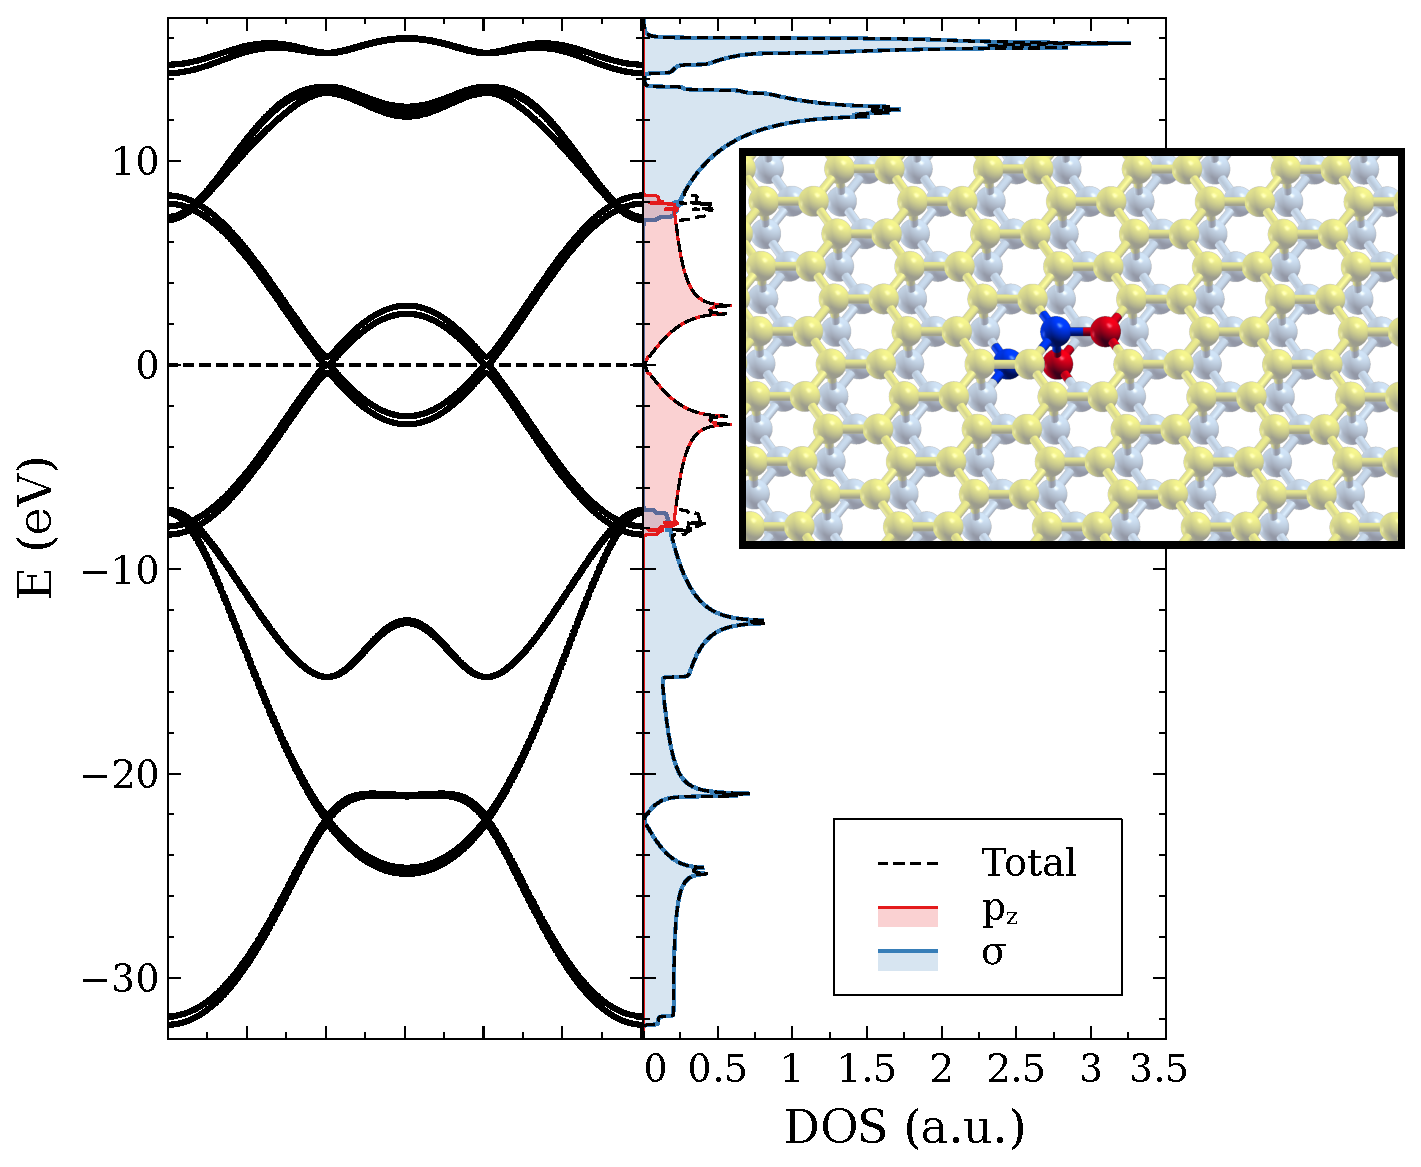
\includegraphics{chapter06/figures/bilayer_bandDOS.pdf}
\vspace{-5pt}
\caption{Band structure and \ac{dos} of bilayer graphene. The red shadowed region shows the contribution of the $p_z$ manifold.}
\label{bilayer}
\end{figure}
\FloatBarrier
%~~~~~~~~~~~~~~~~~~~~~~~~~~~~~~~~~~~~~~~~~~~~~~~~~~~~~~~~~~~%
The $p_z$ bands at the $K$ point are split by an amount proportional to the interlayer hopping

Notice that in the bilayer the $p_z$ manifold is no longer decoupled from the rest of the orbitals (for instance there is a finite hopping between $p_z$ orbitals from one layer and $s$ orbitals of the other), nevertheless close to the Fermi energy the approximation of considering only $p_z$ orbitals is still justified.
The general aspect of the \ac{dos} is similar to that of the graphene but it is important to notice that at $E=0$ the \ac{dos} is now finite.

 \section{Effect of the electric field}
The main effect of an external electric field applied to bilayer graphene is to shift the (on-site) energy of the electrons, we can write such a Hamiltonian term like

\begin{equation}
  H_{\vec{E}} = \lambda_{\vec{E}}\sum_i \varepsilon_l \crea{c}{i}\des{c}{i}
\end{equation}
where $\varepsilon_l=\pm1$ depending on the layer, $l$,  of the atom $i$.
The effect of such a term in \ac{gb} is just to open a gap close to the Fermi energy as shown in fig~\ref{bi_Efield}.

%~~~~~~~~~~~~~~~~~~~~~~~~~~ FIGURE ~~~~~~~~~~~~~~~~~~~~~~~~~%
\begin{figure}[h!]
  \centering
  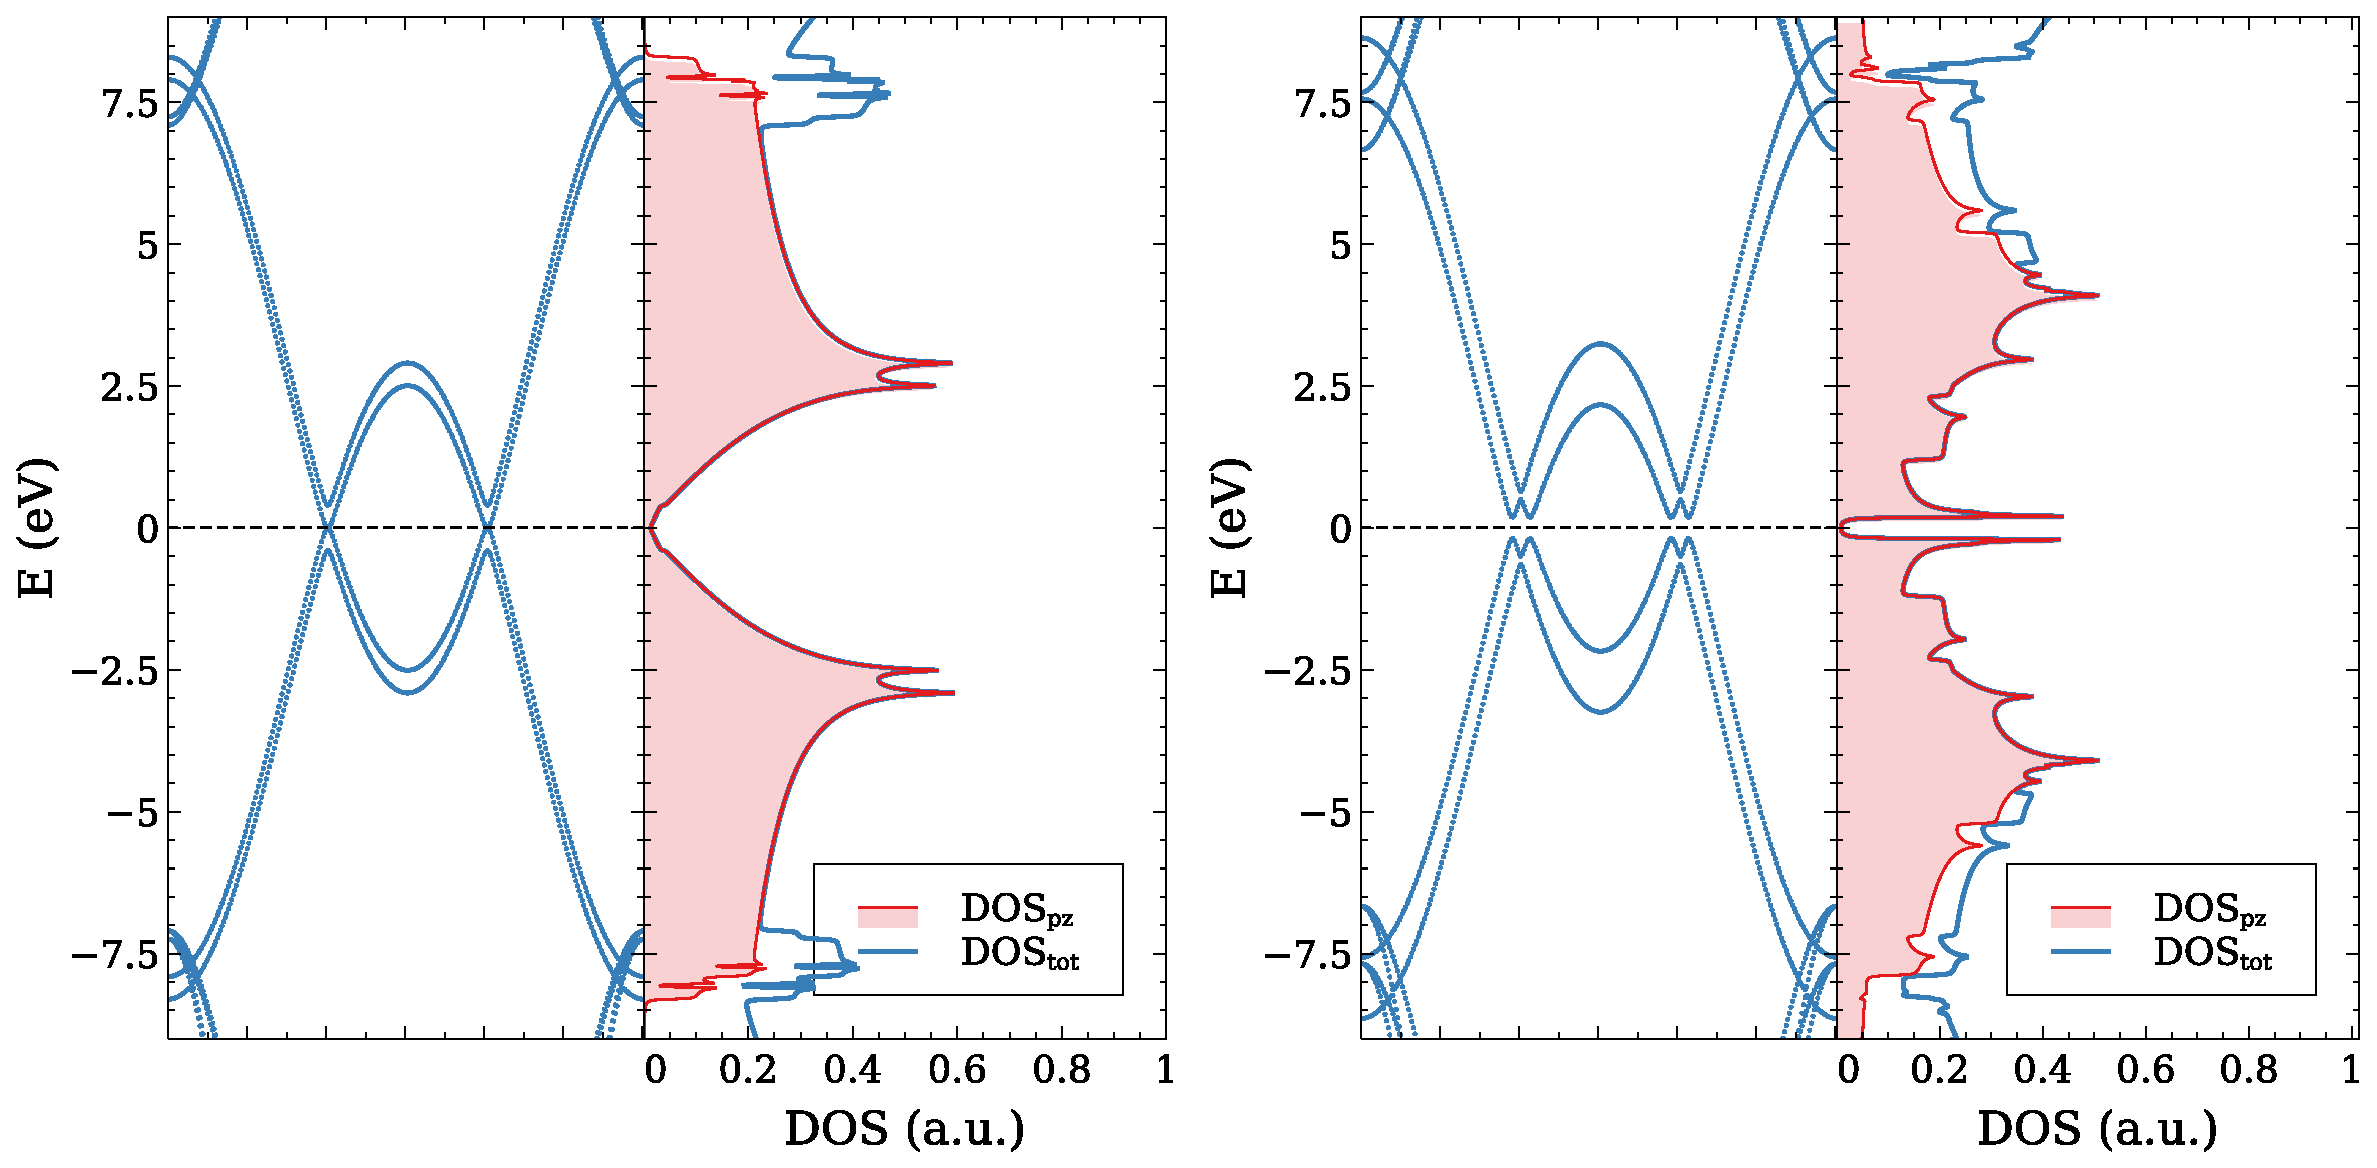
\includegraphics[width=\textwidth]{chapter06/figures/bilayer_elec.pdf}
  \vspace{-10pt}
  \caption{\ac{dos} of a bilayer graphene system in the absence (left panel) and presence (right panel) of an electric field $E=\SI{0.5}{\eV}$.} %XXX UNITS
  \label{bi_Efield}
\end{figure}
\FloatBarrier
%~~~~~~~~~~~~~~~~~~~~~~~~~~~~~~~~~~~~~~~~~~~~~~~~~~~~~~~~~~~%

% Analogously to the discussed scenario of a vacancy in (monolayer) graphene, the introduction of a vacancy also results in the appearance of a ``zero energy state''. In the presence of an external electric field the impurity state will not appear at $E=0$ but shifted in energy as shown in fig.~\ref{dos_bi_dfct}

% %~~~~~~~~~~~~~~~~~~~~~~~~~~ FIGURE ~~~~~~~~~~~~~~~~~~~~~~~~~%
% \begin{figure}[h!]
% \centering
% 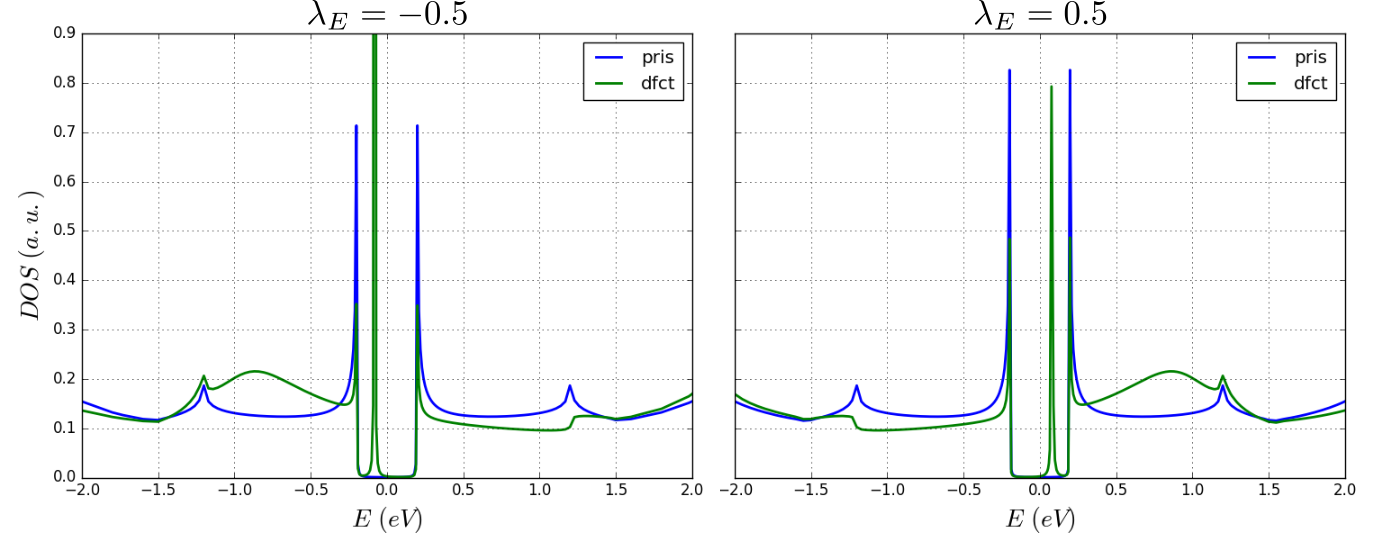
\includegraphics{chapter06/figures/bilayer_dos_dfct.png}
% \vspace{-5pt}
% \caption{\ac{dos} of bilayer graphene with (green line) and without (blue line) a vacancy in the presence of an external electric field. The left and right panels have been calculated for electric fields of opposite sign, notice that }
% \label{dos_bi_dfct}
% \end{figure}
% \FloatBarrier
% %~~~~~~~~~~~~~~~~~~~~~~~~~~~~~~~~~~~~~~~~~~~~~~~~~~~~~~~~~~~%

\subsection{About the charge neutrality}
when a bias is applied to \ac{gb} there is the chance that some charge is transferred form one layer to the other\cite{Wang2016a,Zhang2009}. To be sure of how relevant this effect is we calculate where the Fermi Energy lies as well as the charge in each layer.



% % The position where the adatom is introduced now is important since one of the sublattices of each layer is fully connected to the other layer. All the possibilities for the H chemisorption are depicted in figure\red{FIG}. We will consider only the structure (b).
% %
% % %~~~~~~~~~~~~~~~~~~~~~~~~~~ FIGURE ~~~~~~~~~~~~~~~~~~~~~~~~~%
% % \begin{figure}[h!]
% % \centering
% % 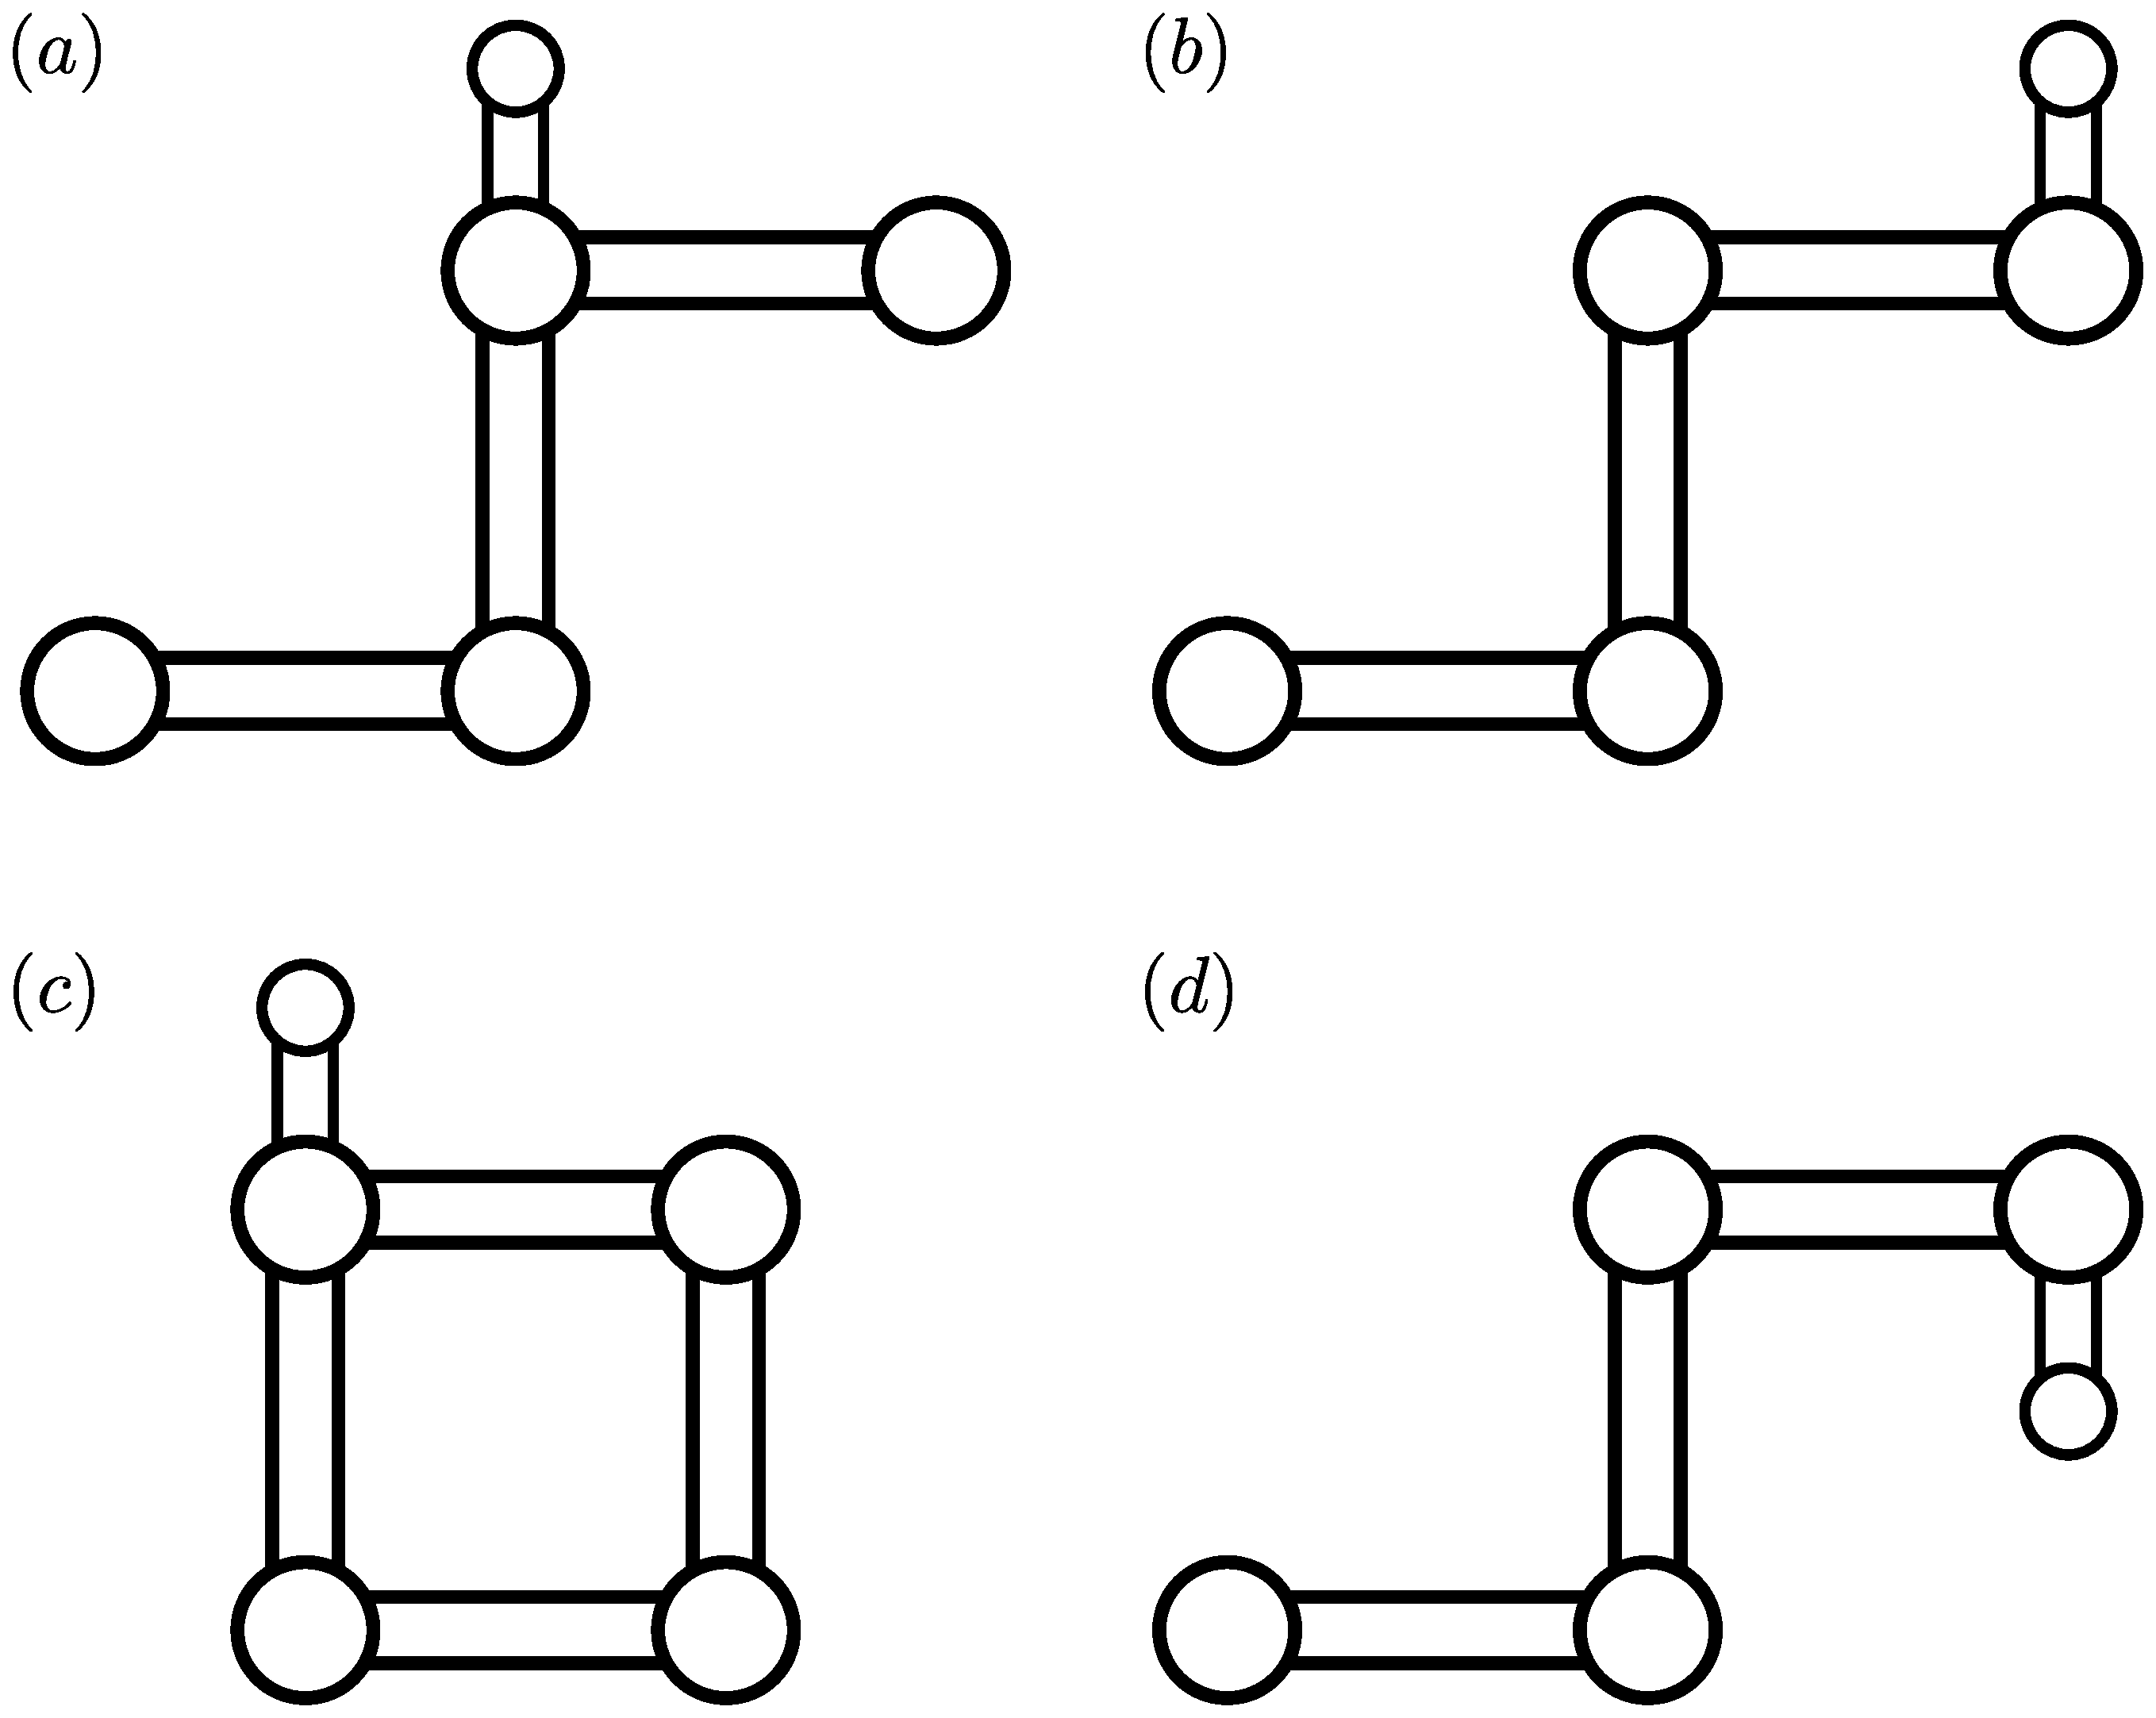
\includegraphics{chapter06/figures/bilayer_H.pdf}
% % \vspace{-5pt}
% % \caption{All opssible atomic strucutre for chemisorbed H}
% % \end{figure}
% % %~~~~~~~~~~~~~~~~~~~~~~~~~~~~~~~~~~~~~~~~~~~~~~~~~~~~~~~~~~~%
% %
% %
% %
% % \subsection{Electric control of the hyperfine interaction}
% % Electric control of the hyperfine with the bias in the bilayer.
% % %~~~~~~~~~~~~~~~~~~~~~~~~~~ FIGURE ~~~~~~~~~~~~~~~~~~~~~~~~~%
% % \begin{figure}[h!]
% % \centering
% % 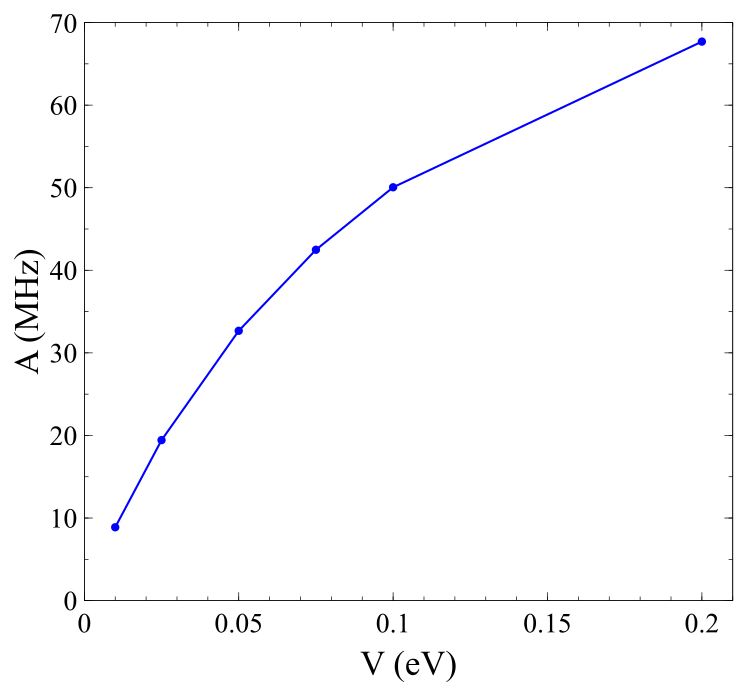
\includegraphics{chapter06/figures/hyperfine.png}
% % \vspace{-5pt}
% % \caption{Hyperfine dependence with the bias voltage.}
% % \end{figure}
% % \FloatBarrier
% % %~~~~~~~~~~~~~~~~~~~~~~~~~~~~~~~~~~~~~~~~~~~~~~~~~~~~~~~~~~~%
% %
% % A similar behavior can be seen from the gap.
% % %~~~~~~~~~~~~~~~~~~~~~~~~~~ FIGURE ~~~~~~~~~~~~~~~~~~~~~~~~~%
% % \begin{figure}[h!]
% % \centering
% % 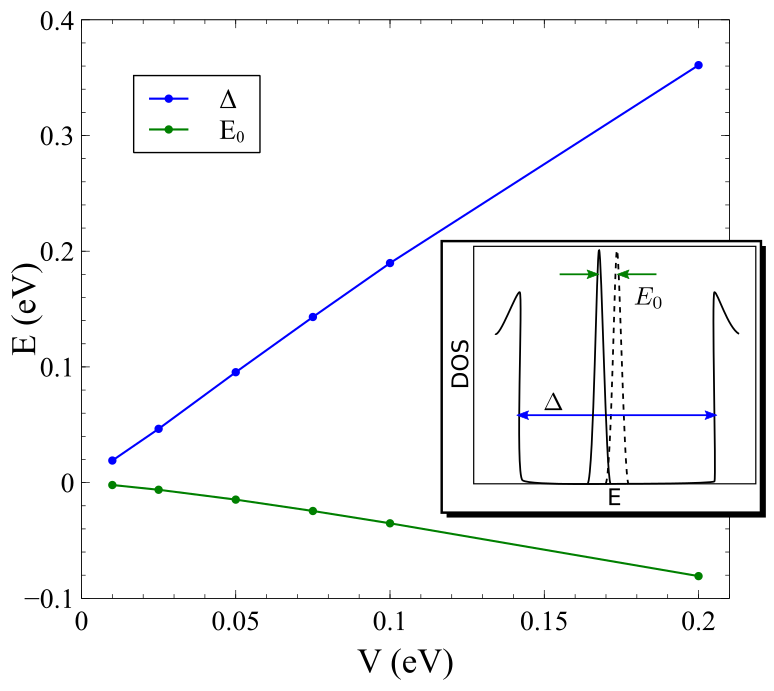
\includegraphics{chapter06/figures/gap.png}
% % \vspace{-5pt}
% % \caption{Dependence of the gap and the energy of the resonance with the bias voltage.}
% % \end{figure}
% % \FloatBarrier
% % %~~~~~~~~~~~~~~~~~~~~~~~~~~~~~~~~~~~~~~~~~~~~~~~~~~~~~~~~~~~%
% %
% %
\section{1 Hydrogen adatom}
\subsection{General considerations} %~~~~~~~~~~~~~~~~~~~~~~~~~~~~~~~~~~~~~~~~~~%
Everything here is done in an armchair island of bilayer graphene, as such, the system is $0$-D, so there is no translational symmetry and no $\vec{k}$ vector can be defined.

To study these systems we will consider a basis of localized states that could be considered to be the $p_z$ hydrogenoid orbitals.
\begin{equation}
  \mathcal{B} = \left\{\phi_1,\phi_2,\dots,\phi_\beta,\dots,\phi_{N_C}\right\}
\end{equation}

Written in such a basis, the general Hamiltonian and its eigenvectors, then, will look like
\begin{equation}
  H = H_t + H_{\lambda_E} \quad\quad;\quad\quad
  H\ket{\psi_\alpha} = E_\alpha\ket{\psi_\alpha} \quad\quad;\quad\quad
  \ket{\psi_\alpha} = \sum_\beta c_\beta\ket{\phi_\beta}
\label{general}
\end{equation}


The term $H_t$ represents the kinetic energy arising from the hopping between neighboring sites and the term $H_{\lambda_E}$ corresponds to the effect of an external electric field on the electrons. Such a term takes the form:
\begin{equation}
  H_{\lambda_E} = \lambda_E
  \left(\begin{array}{cc}
  \mathds{1} & 0 \\
  0 & -\mathds{1}
  \end{array}\right)
\end{equation}
where the elements $\pm\mathds{1}$ refer to the identity for the upper and lower layer respectively.

The vacancies are introduced in this model as an infinite on-site energy for the chosen atom(s). Unless otherwise stated everything is done in $\si{\eV}$ %$eV$
, \emph{not hopping units}, the $p_z$-$p_z$ hopping is chosen as $t=\SI{-2.7}{\eV}$.





\subsection{Note on the geometry}
Any vacancy considered will always be chosen on a hollow position (see fig~\ref{geo_sketch} $c)$) even if it not specified in the text.

When only one vacancy is considered, it will be placed at the atomic position closest to the center of the island.

When two vacancies are considered they will be placed as separated from the edges as possible, as shown in fig~\ref{geo_sketch} $b)$ since this configuration allows the study of a wider range of the parameters $\alpha$ and $d$. Later in the text another configuration consisting in one vacancy in the center of the island, and the other in different positions $\vec{r}=d\cos(\alpha)+d\sin(\alpha)$.
%~~~~~~~~~~~~~~~~~~~~~~~~~~ FIGURE ~~~~~~~~~~~~~~~~~~~~~~~~~%
\begin{figure}[h!]
\centering
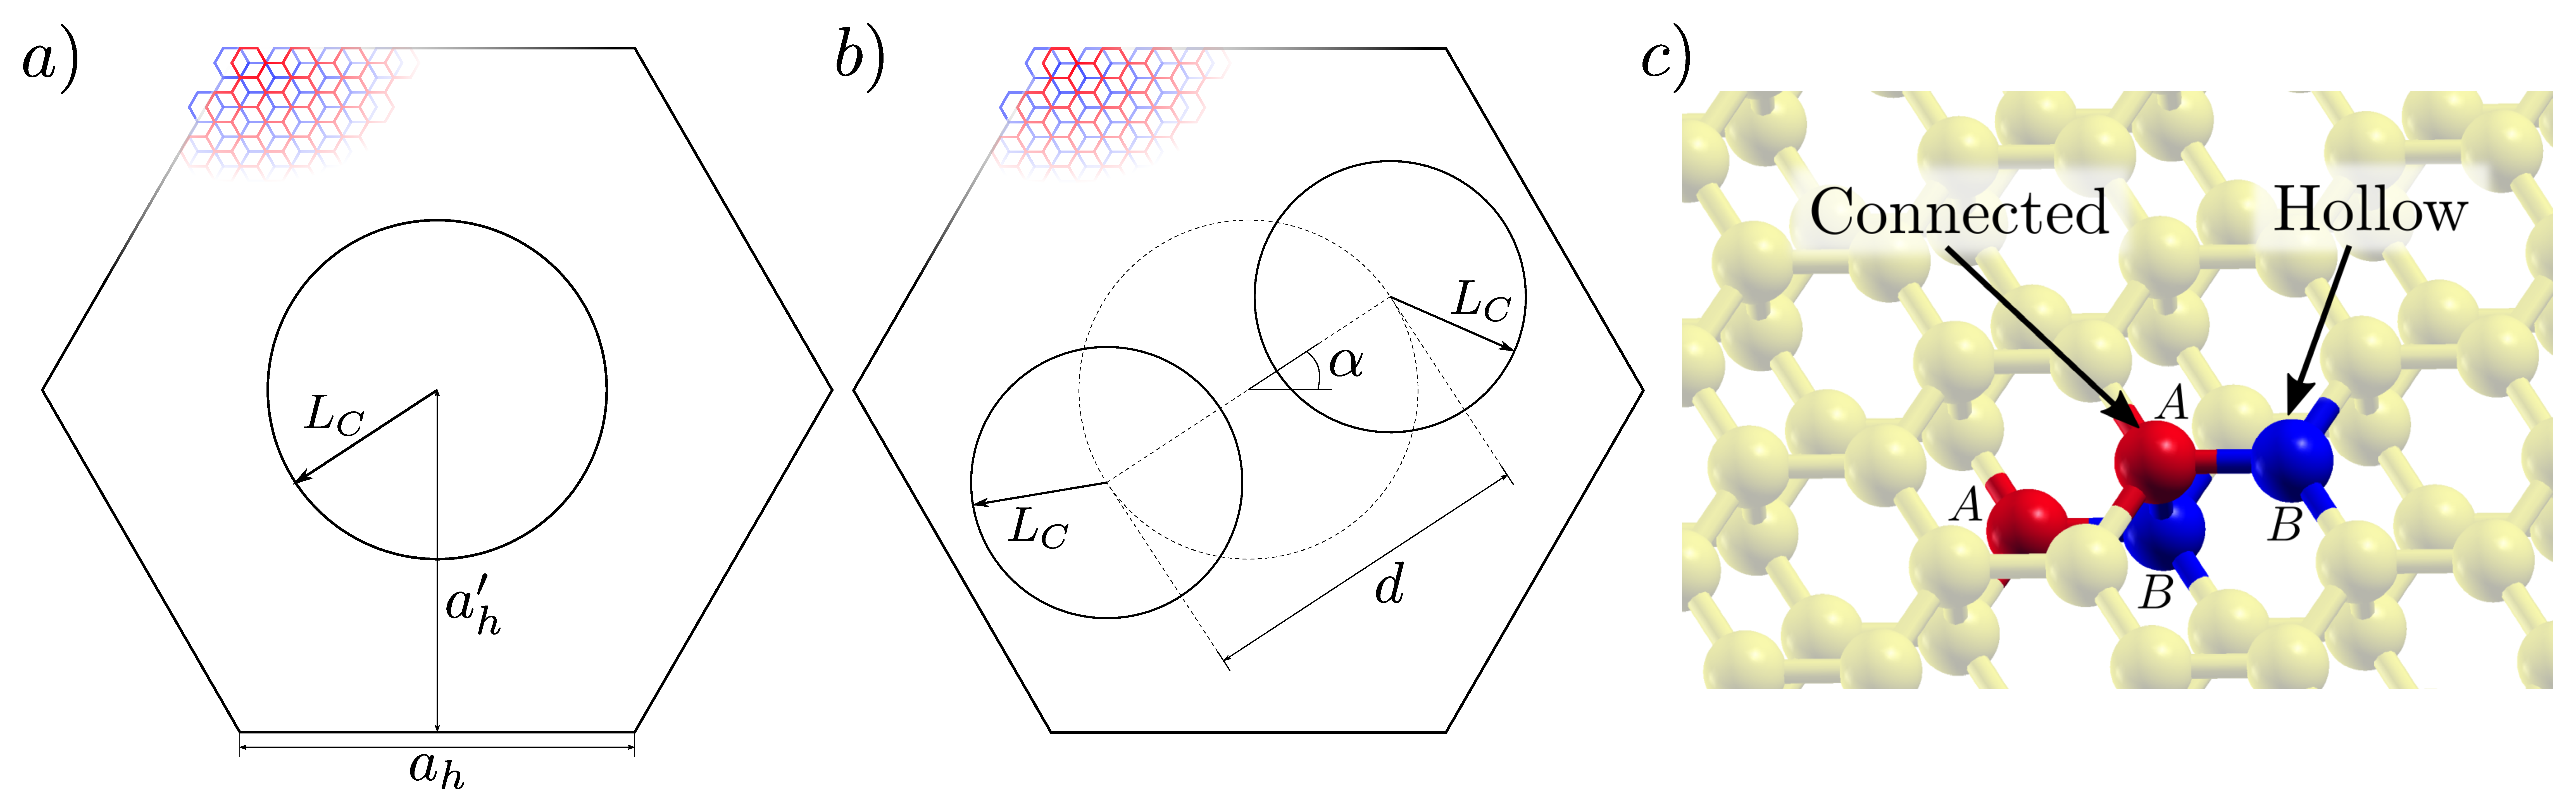
\includegraphics[width=\textwidth]{chapter06/figures/vacs_sketch.pdf}
\vspace{-15pt}
\caption{$a)$ and $b)$ show sketches of the position of the vacancies and relevant geometric information. In the upper left corner the real atomic structure is shown using blue for the lower layer and red for the upper one. The length $L_C$ is the typical size of the in-gap state. $c$ atomic structure showing the ``connected'' and ``hollow'' sites in the upper layer as well as the $A/B$ sublattices (in red/blue).}
\label{geo_sketch}
\end{figure}
\FloatBarrier
%~~~~~~~~~~~~~~~~~~~~~~~~~~~~~~~~~~~~~~~~~~~~~~~~~~~~~~~~~~~%

Note that as long as the border effects are negligible, and due to the $C_3$ symmetry of the in-gap states in graphene, we only need to explore the range of angles between vacancies of $\alpha\in\left[0,60\right]$.


\subsection{Single vacancy} %~~~~~~~~~~~~~~~~~~~~~~~~~~~~~~~~~~~~~~~~~~~~~~~~~~%
Since we are studying an island with a single vacancy, the energy levels are a discrete set of energies. In figure~\ref{1vac_spec} (c) the difference in the spectrum due to the introduction of a vacancy at $\lambda_E=0$ is shown. When a vacancy is introduced, an in-gap state appears at $E=0$ and some \emph{(quasi-)}degeneracies are broken.

The effect of the electric field in the spectrum is shown in figure~\ref{1vac_spec} $a)$ and $b)$. Its main effect is to open a gap, linearly dependent with the electric field.

The shift in the energy at which the in-gap state appears is linear for low electric field, but it remains in-gap for all the regime of electric fields studied. In fig~\ref{1vac_spec} $a$-$c)$ only the eight eigenvalues closest to $E=0$ are plotted. Nevertheless, since the spacing between levels is much smaller than the gap open by the electric field, they appear grouped in two sets of almost-degenerate energies, one at $E>0$ and the other at $E<0$.\\

%~~~~~~~~~~~~~~~~~~~~~~~~~~ FIGURE ~~~~~~~~~~~~~~~~~~~~~~~~~%
\begin{figure}[!ht!]
\centering
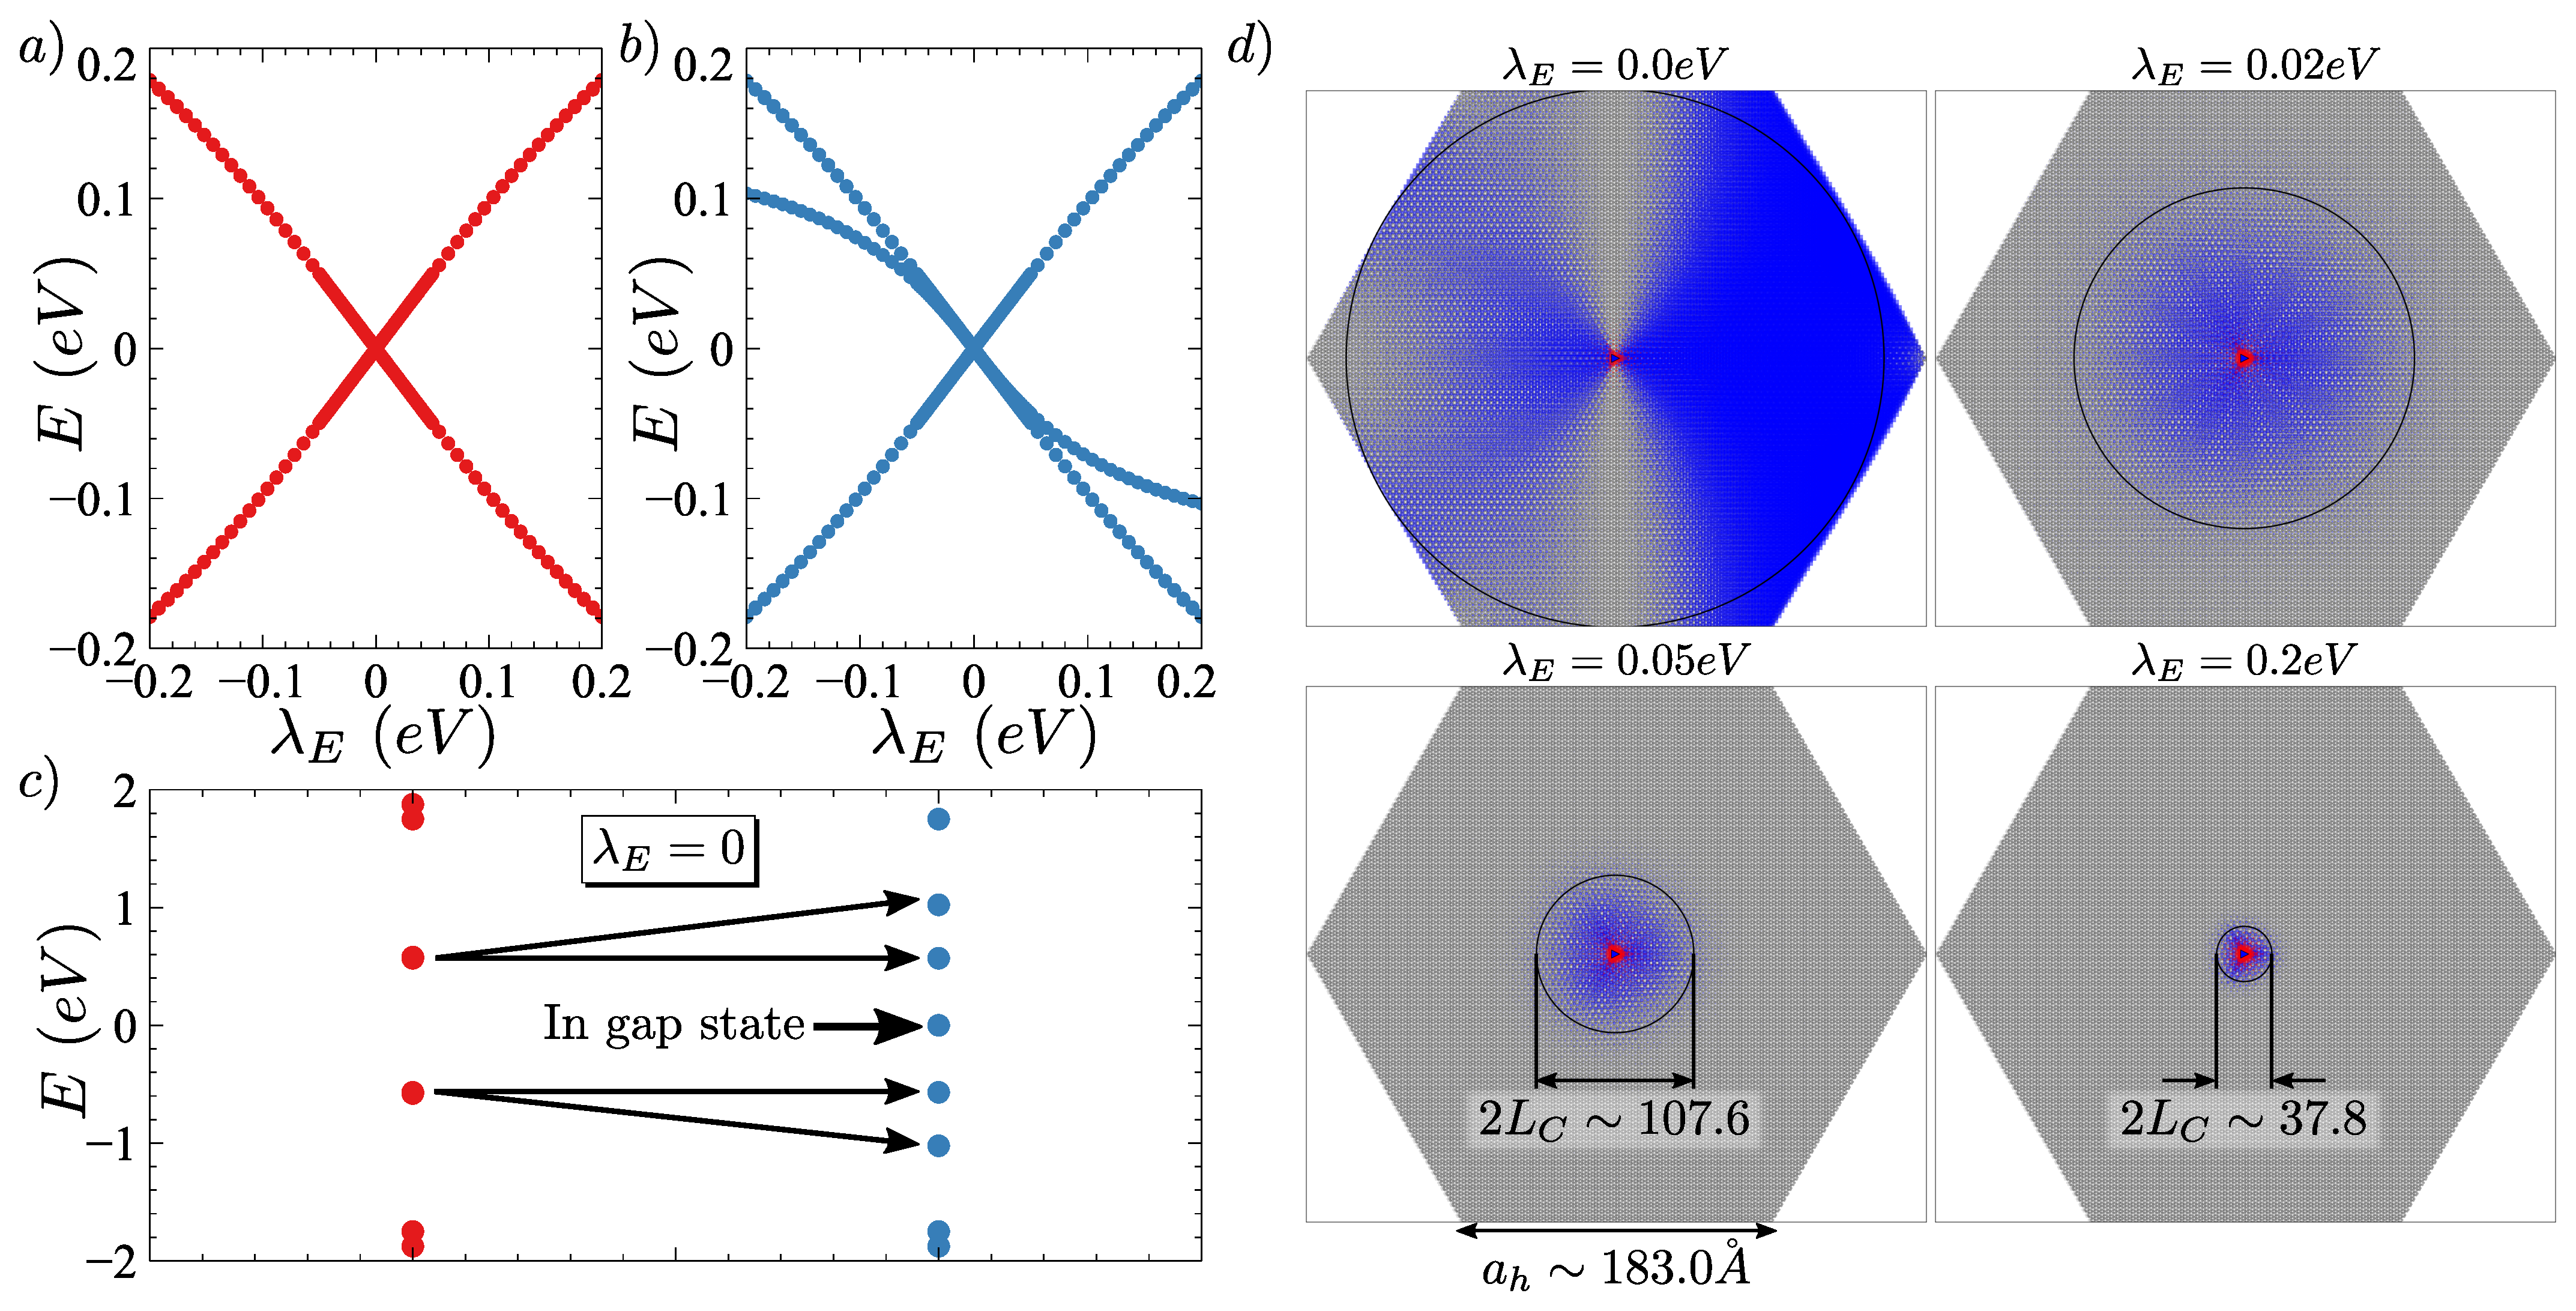
\includegraphics[width=\textwidth]{chapter06/figures/single_vac_spectrum.pdf}
\vspace{-15pt}
\caption{$a)$ and $b)$ show the pristine and defected spectrum respectively as a function of different applied electric fields. Notice the opening of a gap linear with the electric field (in both the pristine and defected cases) and the appearance of an extra state inside the gap. $c)$ Pristine (red) and defected (blue) spectrum for the case of no electric field $\lambda_E=0$. Panel $d)$ shows four snapshots of an island ($N_C=91812$ atoms) at different values of the electric field. The black circle in panel $d)$ shows the confinement length $L_C$ defined in the text.}
\label{1vac_spec}
\end{figure}
\FloatBarrier
%~~~~~~~~~~~~~~~~~~~~~~~~~~~~~~~~~~~~~~~~~~~~~~~~~~~~~~~~~~~%

In Fig~\ref{1vac_spec} $d)$ we show four snapshots of the spatial distribution of the in-gap state. The actual lattice of the island is shown as black dots (probably indistinguishable because of the size of the image).
On top of each atomic position the weight of the wave function ($|c_\beta|^2$ using the notation of eq.~\eqref{general}) is plotted in blue/red for the lower/upper layer.
On top of all this, the site of the vacancy is marked with a blue triangle.
As a visual guide the confinement length is plotted as a black circle with diameter $2L_C$.\\

At $\lambda_E=0$ the system is bipartite, so according to the Lieb's theorem, after the removal of one site, a sublattice-polarized state should appear at $E=0$. This is exactly what happens as shown in Fig.~\ref{1vac_spec}.

When we study the real-space distribution of the in-gap state we find that in the absence of electric field ($\lambda_E=0$) the state is spread all over the island, Fig.~\ref{1vac_spec} $d)$, no matter the size of the island (see Fig.~\ref{IPR_lc} $a)$ bellow). Notice that the effect of the border is not negligible in this regime and, in fact, is the responsible of the breaking of the expected $C_3$ symmetry of the state (at long distances, close to the vacancy the $C_3$ symmetry is almost preserved).


Another important aspect is that the distribution of this wave function is such that in the upper layer (the one containing the vacancy) the wave function is quite confined around the vacancy (3-6 closest atoms) and it barely changes with the electric field, whereas in the lower layer the spreading of the wave function varies from the whole space available, to a few angstroms.


To study quantitatively the properties of the in-gap state $\psi_0$ we define four quantities that will be useful later on.
\begin{itemize}
  \item \emph{Confinement length}, $L_C$, defined, hand-wavingly, as the distance at which more than $90\%$ of the state is located
  \begin{equation}
    0.9 = \int_{0}^{L_C} \psi_0(r) dr   %XXX arreglar!!!
    \label{loclen}
  \end{equation}
  This confinement length can be used as a measurement of the spreading of the in-gap state $\psi_0$.
  \item \emph{Inverse participation ratio} (IPR), $\eta$. Using the notation of equation~\eqref{general}, the IPR can be defined as:
  \begin{equation}
    \ket{\psi_0} = \sum_\beta c_\beta\ket{\phi_\beta}\quad\quad;\quad\quad
    \text{IPR} = \eta = \sum_i |c_\beta|^4
  \end{equation}
  \item \emph{Sublattice} and \emph{Layer polarization}, defined as the expected value of the in-gap state.
  \begin{equation}
    SP = \bra{\psi_0}\widehat{\mathcal{S}}\ket{\psi_0}
    \quad\quad;\quad\quad
    SL = \bra{\psi_0}\widehat{\mathcal{L}}\ket{\psi_0}
  \end{equation}
  where the operators $\widehat{\mathcal{S}}$ and $\widehat{\mathcal{L}}$ measure the component of a given state in a given sublattice and layer respectively. Both $SP$ and $SL$ have to be, by definition, in the closed interval $\left[-1,1\right]$.
\end{itemize}

In figure~\ref{IPR_lc} we study the dependence of these four properties, for different sizes of the island, as a function of the electric field.
%~~~~~~~~~~~~~~~~~~~~~~~~~~ FIGURE ~~~~~~~~~~~~~~~~~~~~~~~~~%
\begin{figure}[!ht]
\centering
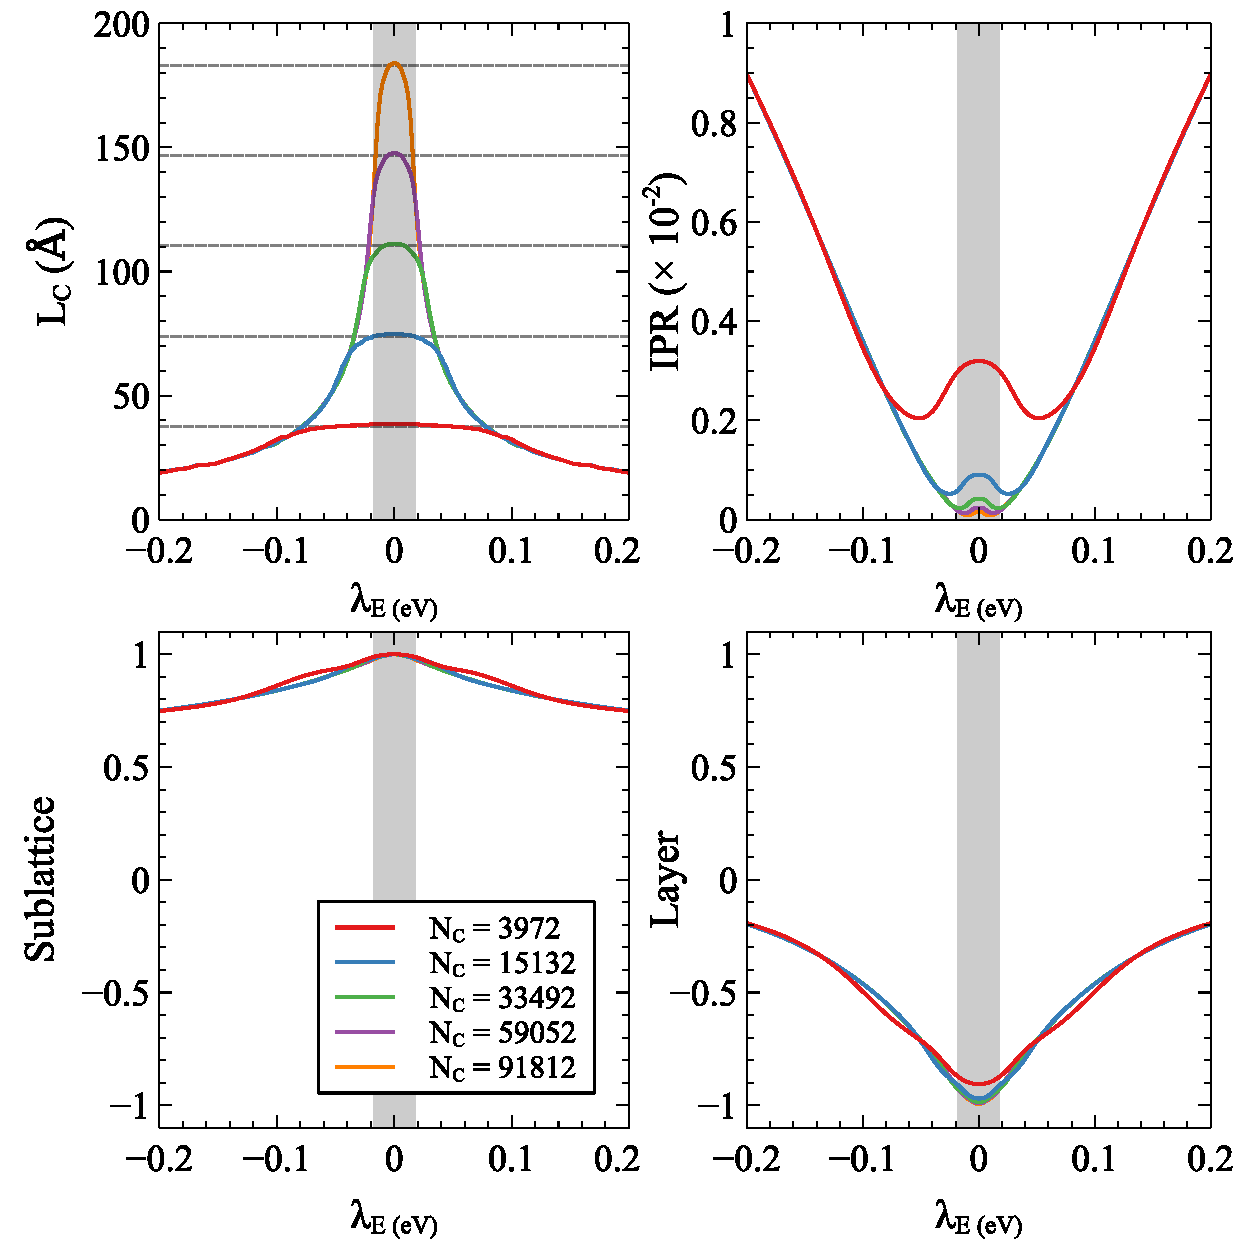
\includegraphics[width=0.6\textwidth]{chapter06/figures/single_vac_properties.pdf}
\vspace{-5pt}
\caption{$a)$ Dependence of the localization length $L_c$ with the electric field for different sizes of the island. The dashed lines corresponds to the size of the each corresponding island. $b)$ IPR, $\eta$, dependence with the electric field for different sizes of the island. $c)$ and $d)$ show the degree of sublattice and layer polarization for different sizes of the island as a function the electric field. The values $\pm1$ refer to $A/B$ sublattice or up/down layer respectively.}
\label{IPR_lc}
\end{figure}
\FloatBarrier
%~~~~~~~~~~~~~~~~~~~~~~~~~~~~~~~~~~~~~~~~~~~~~~~~~~~~~~~~~~~%

It can be seen in Fig.~\ref{IPR_lc} $a)$ that as we approach the limit $\lambda_E\rightarrow0$ the confinement length collapses to the size of the island, shown as a dashed line for each size studied. This plateau is just the effect of having an in-gap state spread all over the island.

The shadowed region in all the panels shows the range of $\lambda_E$ in which the border effects can be relevant for the biggest island studied ($N_C=91812$). It is estimated as the $\lambda_E$ at which the results differ from those of the previous island. Of course it is only a rough estimation and it should be considered only as a guide to the eye when reading the results.

In panel $b)$ the IPR is shown. Except for small islands the evolution of the IPR, as that of the $L_C$, is the same regardless of the size of the island. The increasing of the IPR with the electric field is another sign of the increasing localization of the in-gap state around the vacancie.\\

The sublattice and layer polarization are shown in panels~\ref{IPR_lc} $c)$ and $d)$. As it can be seen at $\lambda_E=0$ the state is completely sublattice-polarized, in accordance with the Lieb's theorem, and almost layer-polarized, this almost is more easly visible in the small red component present in Fig.~\ref{1vac_spec} $d)$.

As the electric field increases the bipartite character of the system is lost, in agreement with the shift of the energy of the in-gap state (no longer at $E=0$). Since the system is no longer bipartite, the sublattice polarized character of the in-gap state is no longer assured, and as shown in panel $c)$ it, in fact, decreases.

The decreasing of the layer polarization is easily understood by looking at Fig.~\ref{1vac_spec} $d)$. For small $\lambda_E$ the in-gap state is mostly spread over the lower layer, while for large $\lambda_E$ the in-gap state occupies roughly the same area in both layers resulting in a $\bra{\psi_0}\widehat{\mathcal{L}}\ket{\psi_0} \rightarrow 0$

% It is to be expected that if two vacancies are placed much closer than $r\sim60\text{angs}$, they could interact strongly rendering its isolation impossible even with big electric fields.



\section{Double vacancy}
it may be possible to control the interaction between two vacancies via an electric field by placing them at a certain distance $d$. First we are going to analyze the general phenomenology of the system studying the different states that appear as a function of the distance and angle between vacancies and the electric field.

%~~~~~~~~~~~~~~~~~~~~~~~~~~ FIGURE ~~~~~~~~~~~~~~~~~~~~~~~~~%
\begin{figure}[h!]
\centering
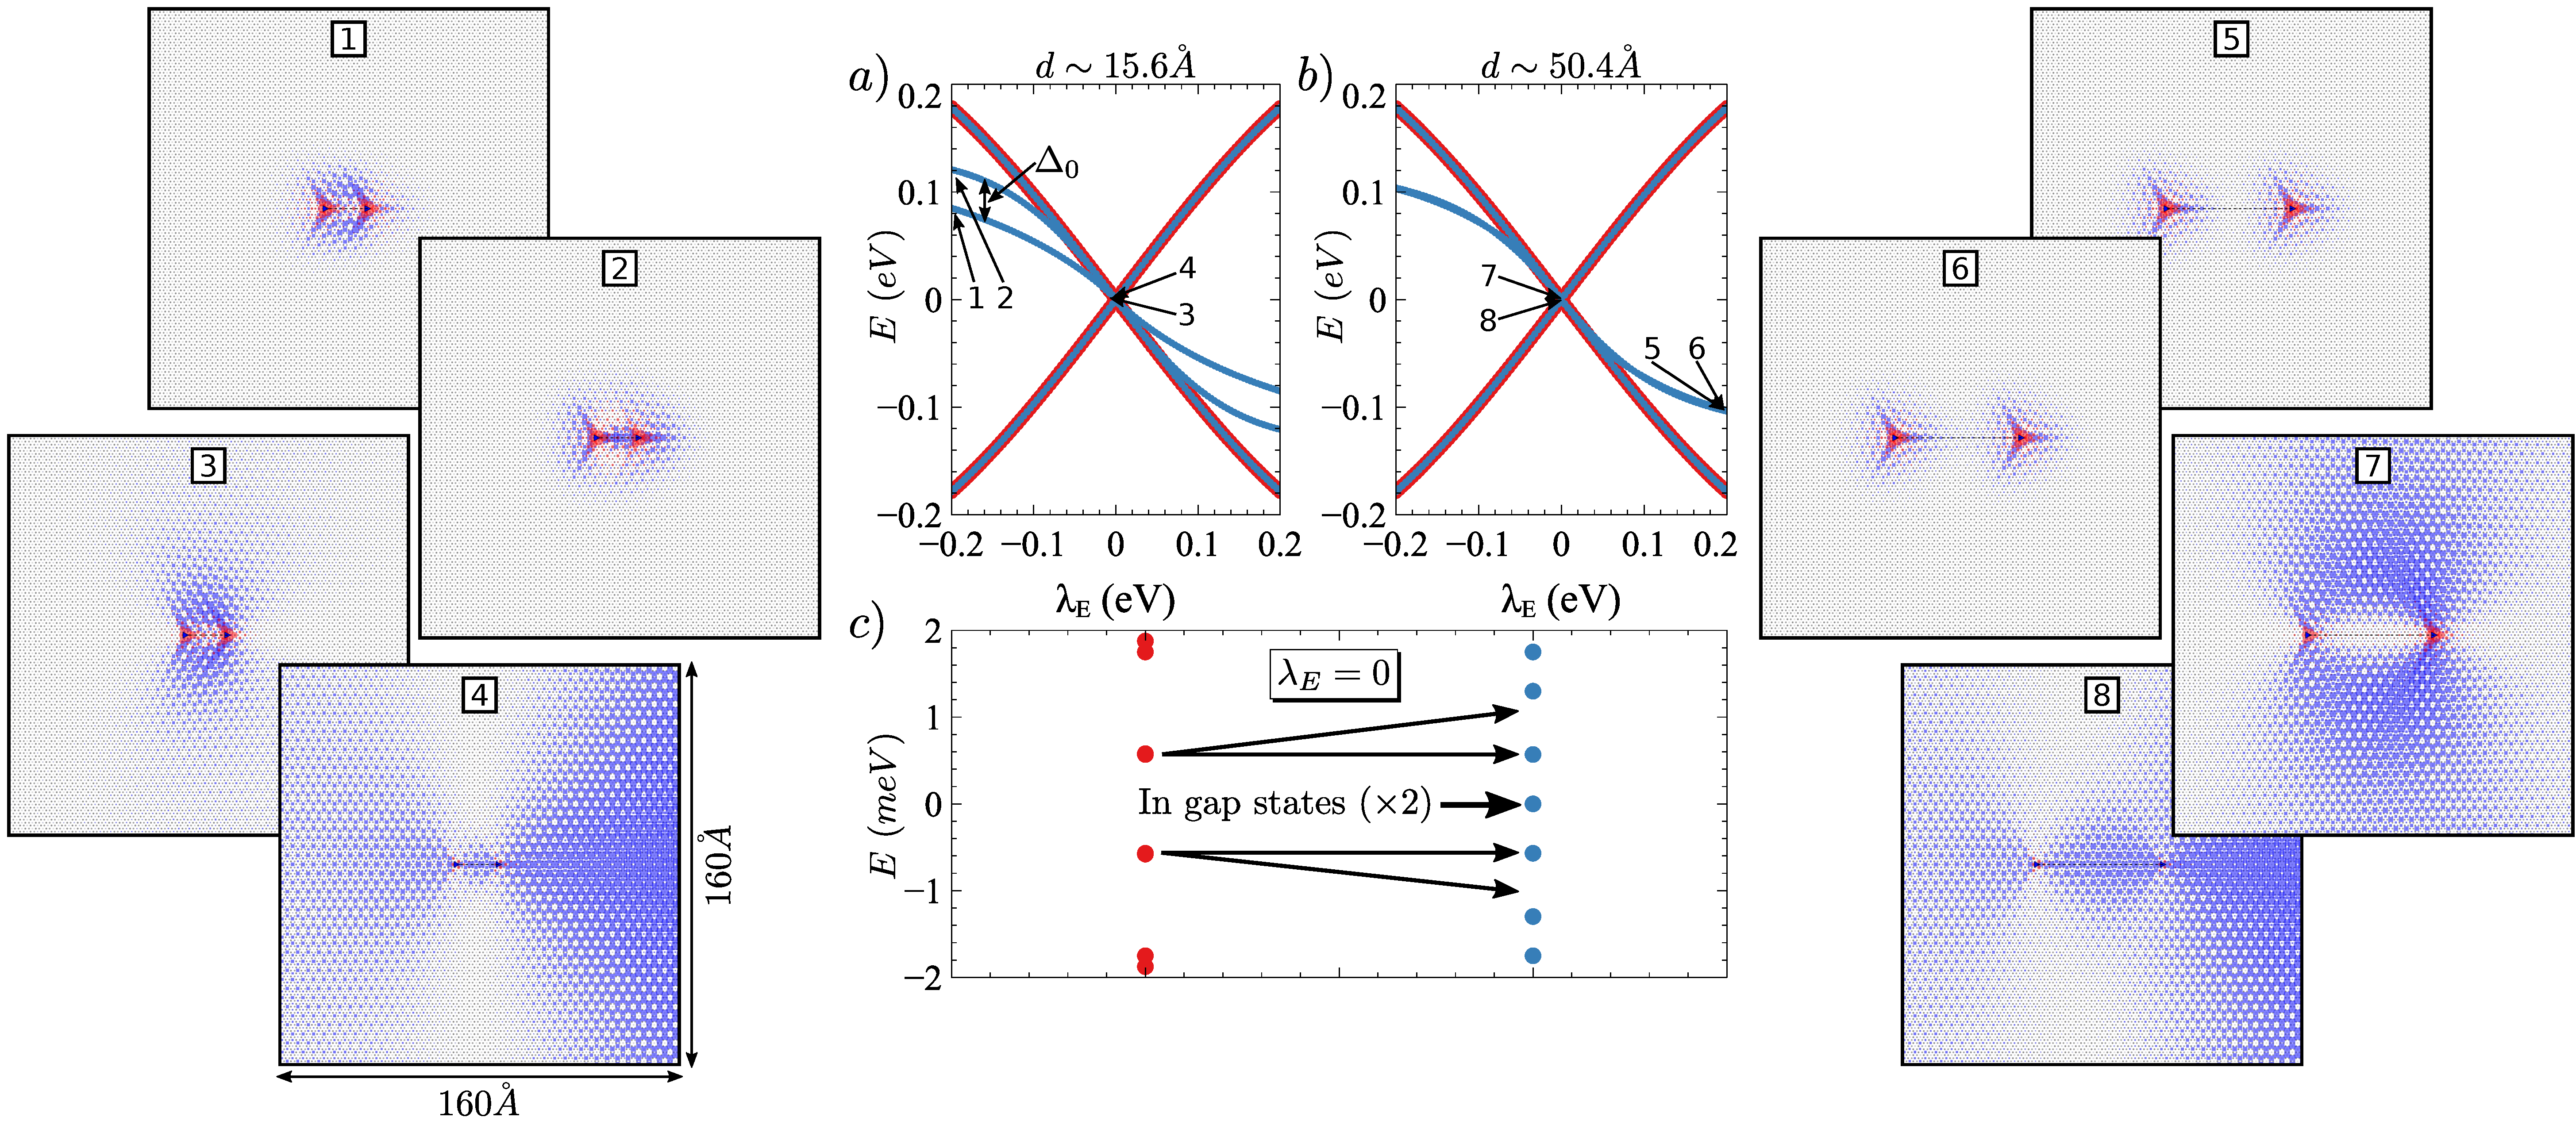
\includegraphics[width=\textwidth]{chapter06/figures/double_vac_spectrum.pdf}
\vspace{-5pt}
\caption{$a)$ and $b)$ show the pristine (red dots) and defected (blue) spectrum as a function of applied electric field. Notice the opening of a gap linear with the electric field (in both the pristine and defected cases) and the appearance of two extra states inside the gap. $c)$ Pristine (red) and defected (blue) spectrum for the case of no electric field $\lambda_E=0$. Notice that the removal of two sites (in the same sublattice) results in two states degenerate at $E=0$. The panels $1$-$8$ show a closer look ($160\times160\text{\AA}$ region) of the spatial distribution of the \emph{in-gap states} for different electric fields $\lambda_E\in\left\{-0.2,0.0,0.2\right\}$.}
\label{2vac_spec}
\end{figure}
\FloatBarrier
%~~~~~~~~~~~~~~~~~~~~~~~~~~~~~~~~~~~~~~~~~~~~~~~~~~~~~~~~~~~%

In the absence of electric field, $\lambda_E = 0$, when two vacancies are introduced in the same sublattice (since both of them have to be in hollow positions) two states appear at $E=0$ in accordance to the Lieb's Theorem as shown in Fig.~\ref{2vac_spec} $c)$. These states are sublattice-polarized and they are mostly located in the lower layer.\\

When we switch on the electric field the spectrum opens a gap that increases linearly with the electric field but the two states associated with the vacancies remain inside the gap.

If the vacancies are close enough to each other the interaction between them is big enough to split this levels (originally degenerate at $E=0$) as shown in Fig.~\ref{2vac_spec} $a)$. In this case in which the vacancies are close, it is apparent from the spatial distribution of the wave functions (panels 1-8) that a pair of bonding-antibonding states is created.

If the distance is between the vacancies is big enough the splitting between the in-gap states becomes negligible as shown in Fig.~\ref{2vac_spec} $b)$. Notice that panels 5 and 6 correspond to the two in-gap eigenstates, $\psi_0$ and $\psi_1$ of the Hamiltonian which are almost degenerate in energy. For that electric field ($\lambda_E=0.2$) the confinement length of these states is smaller than the distance between the vacancies, which explains why they barely interact and are, therefore, degenerate in energy.



\subsection{Spin Exchange Interactions} %~~~~~~~~~~~~~~~~~~~~~~~~~~~~~~~~~~~~~~%
Starting from the notes on the effective exchange, equations 9 and 10. I focus for now on the effective coupling $J$.

Let's remember that for getting to that formula we start from two in-gap states that should be associated to each of the vacancies.
In our case, the in-gap states, $\psi_0$ and $\psi_1$, take the form of bonding-antibonding states, hence we can define a left $\psi_L$ and right $\psi_R$ states as:
\begin{equation}
  \psi_L = \frac{1}{2}\left(\psi_0 \pm \psi_1\right) \quad\quad;\quad\quad
  \psi_R = \frac{1}{2}\left(\psi_0 \mp \psi_1\right)
\end{equation}
The sign of this definition may depend on the numerical diagonalization, and it will be decided such that:
\begin{equation*}
  \bra{\psi_L}X\ket{\psi_L} < \bra{\psi_R}X\ket{\psi_R}
\end{equation*}
where $X$ is the position (in the $X$-axis) operator.


\subsubsection{Anti-ferromagnetic coupling}
The in-gap states can form a bonding-antibonding pair resulting in a splitting of the levels, $\Delta_0$. The Anti-ferromagnetic coupling is defined as
\begin{equation}
  J_{AF} \propto \Delta^2_0     %\frac{\Delta^2_0}{U_{Eff}}
\end{equation}


\subsubsection{Ferromagnetic coupling}
The operator that creates an electron at the atom i with spin $\sigma$ can be written as:
\begin{equation}
  \crea{c}{i\sigma} = \sum_v\psi_v(i)\crea{a}{v_\sigma}+
                      \sum_c\psi_c(i)\crea{a}{c_\sigma}+
                      L^*(i)\crea{a}{L\sigma} + R^*(i)\crea{a}{R\sigma}
\label{creation}
\end{equation}
But we will restrict to the in-gap states manifold, hence we define the creation and destruction operator for an electron with spin $\sigma$:
\begin{equation}
  \crea{c}{i\sigma} = L^*(i)\crea{a}{L\sigma} + R^*(i)\crea{a}{R\sigma}
  \quad\quad;\quad\quad
  \des{c}{i\sigma} = L(i)\des{a}{L\sigma} + R(i)\des{a}{R\sigma}
\end{equation}
With this approximation the density operator $n_{i\sigma} = \crea{c}{i\sigma}\des{c}{i\sigma}$  reads:
\begin{equation}
  \begin{split}
  n_{i\sigma} &= (L^*(i)\crea{a}{L\sigma} + R^*(i)\crea{a}{R\sigma})
                 (L(i)\des{a}{L\sigma} + R(i)\des{a}{R\sigma}) =\\
              &= |L(i)|^2 \crea{a}{L\sigma}\des{a}{L\sigma}+
                 |R(i)|^2 \crea{a}{R\sigma}\des{a}{R\sigma}+
                 L^*(i)R(i)\crea{a}{L\sigma}\des{a}{R\sigma}+
                 R^*(i)L(i)\crea{a}{R\sigma}\des{a}{L\sigma}
  \end{split}
\end{equation}

Now we expand the Hubbard operator,
\begin{equation*}
  H_U = U\sum_i n_{i\uaw}n_{i\daw}
\end{equation*}
dropping the $i$ label
\begin{equation}
  \begin{split}
    n_\uaw n_\daw= &\left[
    |L|^2 \crea{a}{L\uaw}\des{a}{L\uaw}+
    |R|^2 \crea{a}{R\uaw}\des{a}{R\uaw}+
    L^*R\crea{a}{L\uaw}\des{a}{R\uaw}+
    R^*L\crea{a}{R\uaw}\des{a}{L\uaw}
    \right]\cdot\\
    &\left[
    |L|^2 \crea{a}{L\daw}\des{a}{L\daw}+
    |R|^2 \crea{a}{R\daw}\des{a}{R\daw}+
    L^*R\crea{a}{L\daw}\des{a}{R\daw}+
    R^*L\crea{a}{R\daw}\des{a}{L\daw}
  \right]=\\
    =& |L|^4 \crea{a}{L\uaw}\des{a}{L\uaw}\crea{a}{L\daw}\des{a}{L\daw}+
     |R|^4 \crea{a}{R\uaw}\des{a}{R\uaw}\crea{a}{R\daw}\des{a}{R\daw}+
     (L^*R)^2\crea{a}{L\uaw}\des{a}{R\uaw}\crea{a}{L\daw}\des{a}{R\daw}+
     (R^*L)^2\crea{a}{R\uaw}\des{a}{L\uaw}\crea{a}{R\daw}\des{a}{L\daw}+\\
  &+|L|^2|R|^2\crea{a}{L\uaw}\des{a}{L\uaw}\crea{a}{R\daw}\des{a}{R\daw}+
    |L|^2L^*R \crea{a}{L\uaw}\des{a}{L\uaw}\crea{a}{L\daw}\des{a}{R\daw}+
    |L|^2R^*L \crea{a}{L\uaw}\des{a}{L\uaw}\crea{a}{R\daw}\des{a}{L\daw}+\\
  &+|R|^2|L|^2 \crea{a}{R\uaw}\des{a}{R\uaw}\crea{a}{L\daw}\des{a}{L\daw}+
    |R|^2L^*R \crea{a}{R\uaw}\des{a}{R\uaw}\crea{a}{L\daw}\des{a}{R\daw}+
    |R|^2R^*L \crea{a}{R\uaw}\des{a}{R\uaw}\crea{a}{R\daw}\des{a}{L\daw}+\\
  &+L^*R|L|^2\crea{a}{L\uaw}\des{a}{R\uaw}\crea{a}{L\daw}\des{a}{L\daw}+
    L^*R|R|^2\crea{a}{L\uaw}\des{a}{R\uaw}\crea{a}{R\daw}\des{a}{R\daw}+
    L^*RR^*L\crea{a}{L\uaw}\des{a}{R\uaw}\crea{a}{R\daw}\des{a}{L\daw}+\\
  &+R^*L|L|^2\crea{a}{R\uaw}\des{a}{L\uaw}\crea{a}{L\daw}\des{a}{L\daw}+
    R^*L|R|^2\crea{a}{R\uaw}\des{a}{L\uaw}\crea{a}{R\daw}\des{a}{R\daw}+
    R^*LL^*R\crea{a}{R\uaw}\des{a}{L\uaw}\crea{a}{L\daw}\des{a}{R\daw}
  \end{split}
\end{equation}
Using that $n_{L\uaw} = \crea{a}{L\uaw}\des{a}{L\uaw}$ and analogously for $n_{R\uaw}$ and also that $L^*L=|L|^2$ we can rewrite
\begin{equation}
  \begin{split}
    n_\uaw n_\daw =& |L|^4 n_{L\uaw}n_{L\daw}+
     |R|^4 n_{R\uaw}n_{R\daw}+
     (L^*R)^2\crea{a}{L\uaw}\des{a}{R\uaw}\crea{a}{L\daw}\des{a}{R\daw}+
     (R^*L)^2\crea{a}{R\uaw}\des{a}{L\uaw}\crea{a}{R\daw}\des{a}{L\daw}+\\
  &+|L|^2|R|^2 n_{L\uaw}n_{R\daw}+
    |L|^2L^*R n_{L\uaw}\crea{a}{L\daw}\des{a}{R\daw}+
    |L|^2R^*L n_{L\uaw}\crea{a}{R\daw}\des{a}{L\daw}+\\
  &+|L|^2|R|^2 n_{R\uaw}n_{L\daw}+
    |R|^2L^*R n_{R\uaw}\crea{a}{L\daw}\des{a}{R\daw}+
    |R|^2R^*L n_{R\uaw}\crea{a}{R\daw}\des{a}{L\daw}+\\
  &+L^*R|L|^2\crea{a}{L\uaw}\des{a}{R\uaw}n_{L\daw}+
    L^*R|R|^2\crea{a}{L\uaw}\des{a}{R\uaw}n_{R\daw}+
    |L|^2|R|^2\crea{a}{L\uaw}\des{a}{R\uaw}\crea{a}{R\daw}\des{a}{L\daw}+\\
  &+R^*L|L|^2\crea{a}{R\uaw}\des{a}{L\uaw}n_{L\daw}+
    R^*L|R|^2\crea{a}{R\uaw}\des{a}{L\uaw}n_{R\daw}+
    |L|^2|R|^2\crea{a}{R\uaw}\des{a}{L\uaw}\crea{a}{L\daw}\des{a}{R\daw}
  \end{split}
\end{equation}
These 16 terms can be rewritten and grouped as
\begin{equation}
  \begin{split}
    n_\uaw n_\daw&= |L|^4 n_{L\uaw}n_{L\daw}+ |R|^4 n_{R\uaw}n_{R\daw}+\\
  &+|L|^2|R|^2\left(n_{L\uaw}n_{R\daw} + n_{R\uaw}n_{L\daw}+
                    \crea{a}{L\uaw}\des{a}{R\uaw}\crea{a}{R\daw}\des{a}{L\daw}+
                    \crea{a}{R\uaw}\des{a}{L\uaw}\crea{a}{L\daw}\des{a}{R\daw}
              \right)+\\
  &+(L^*R)^2\crea{a}{L\uaw}\des{a}{R\uaw}\crea{a}{L\daw}\des{a}{R\daw}+
     (R^*L)^2\crea{a}{R\uaw}\des{a}{L\uaw}\crea{a}{R\daw}\des{a}{L\daw}+\\
  &+|L|^2L^*R \left(n_{L\uaw}\crea{a}{L\daw}\des{a}{R\daw}+
                   \crea{a}{L\uaw}\des{a}{R\uaw}n_{L\daw}\right)+
    |L|^2R^*L \left(n_{L\uaw}\crea{a}{R\daw}\des{a}{L\daw}+
                   \crea{a}{R\uaw}\des{a}{L\uaw}n_{L\daw}\right)+\\
  &+|R|^2L^*R \left(n_{R\uaw}\crea{a}{L\daw}\des{a}{R\daw}+
                   \crea{a}{L\uaw}\des{a}{R\uaw}n_{R\daw}\right)+
    |R|^2R^*L \left(n_{R\uaw}\crea{a}{R\daw}\des{a}{L\daw}+
                   \crea{a}{R\uaw}\des{a}{L\uaw}n_{R\daw}\right)
  \end{split}
\end{equation}

We can rename the couplings of these terms for an easier interpretation\footnote{the deduction was made for $n_\uaw n_\daw$, but the Hubbard term actually reads $H_U = U\sum_i n_{i\uaw}n_{i\daw}$}:
\begin{equation}
  \begin{split}
    \tilde{U}_L &= U\sum_i |L(i)|^4\\
    \tilde{U}_R &= U\sum_i  |R(i)|^4\\
    \frac{J}{2} &= U\sum_i  |L(i)|^2|R(i)|^2\\
    \Delta &= U\sum_i  (L^*(i)R(i))^2\\
    t_{LR} &= U\sum_i  |L(i)|^2L^*(i)R(i)\\
    t_{RL} &= U\sum_i  |R(i)|^2R^*(i)L(i)
  \end{split}
\label{rename}
\end{equation}
Finally, rearranging the creation and destruction operators and noticing that $\crea{a}{L\uaw}\des{a}{L\daw} = S^+_L$, the Hubbard term can be expressed as the addition of 5 terms
\begin{equation*}
  H_U = H_{\tilde{U}} + H_J + H_{pair} + H_{LR} + H_{RL}
\end{equation*}
with
\begin{equation}
  H_{\tilde{U}} = \tilde{U}_L n_{L\uaw}n_{L\daw}+
                  \tilde{U}_R n_{R\uaw}n_{R\daw}
\end{equation}
\begin{equation}
  H_{J} =\frac{J}{2}\left(n_{L\uaw}n_{R\daw} + n_{R\uaw}n_{L\daw}-
              S^+_LS^-_R - S^+_RS^-_L \right)
\label{Jraw}
\end{equation}
\begin{equation}
  H_{pair} = \Delta \crea{a}{L\uaw}\crea{a}{L\daw}\des{a}{R\uaw}\des{a}{R\daw}+
             \Delta^* \crea{a}{R\uaw}\crea{a}{R\daw}\des{a}{L\uaw}\des{a}{L\daw}
\end{equation}
\begin{equation}
  H_{LR} = t_{LR} \left(n_{L\uaw}\crea{a}{L\daw}\des{a}{R\daw}+
                   \crea{a}{L\uaw}\des{a}{R\uaw}n_{L\daw}\right)+
           t^*_{LR} \left(n_{L\uaw}\crea{a}{R\daw}\des{a}{L\daw}+
                   \crea{a}{R\uaw}\des{a}{L\uaw}n_{L\daw}\right)
\end{equation}
\begin{equation}
  H_{LR} = t_{RL} \left(n_{R\uaw}\crea{a}{L\daw}\des{a}{R\daw}+
                   \crea{a}{L\uaw}\des{a}{R\uaw}n_{R\daw}\right)+
           t^*_{RL} \left(n_{R\uaw}\crea{a}{R\daw}\des{a}{L\daw}+
                   \crea{a}{R\uaw}\des{a}{L\uaw}n_{R\daw}\right)
\end{equation}

\subsection{Heisenberg coupling}
In order to try to make apparent the effective Heisenberg term we first expand the standard Heisengberg Hamiltonian in terms of the density operators.
\begin{equation}
  \mathcal{H}_J = -J\vec{S}_L\cdot\vec{S}_R =
  -J \left[S^z_LS^z_R+\frac{1}{2}\left(S^+_LS^-_R+S^-_LS^+_R\right)\right]
\end{equation}
The Ising contribution, can be written in terms of the density operators by taking into account that $S^z_\alpha = (n_\alpha\uaw-n_\alpha\daw)/2$,

\begin{equation}
  \mathcal{H}_{Ising} = -J S^z_LS^z_R = -\frac{J}{4}
      \left(n_{L\uaw}n_{R\uaw}+n_{L\daw}n_{R\daw}-
            n_{L\daw}n_{R\uaw}-n_{L\uaw}n_{R\daw}\right)
\label{Ising_goal}
\end{equation}
Hence, the Heisenberg Hamiltonian can be written as
\begin{equation}
  \mathcal{H}_J = -J\vec{S}_L\cdot\vec{S}_R =
  -\frac{J}{4}\left(n_{L\uaw}n_{R\uaw}+n_{L\daw}n_{R\daw}-
                    n_{L\daw}n_{R\uaw}-n_{L\uaw}n_{R\daw}\right)
  -\frac{J}{2}\left(S^+_LS^-_R+S^-_LS^+_R\right)
\label{heisenberg_goal}
\end{equation}
Now we make explicit the Heisenberg contribution arising from the effective Hamiltonian~\eqref{Jraw}. To do so we need to take into account the following constrain:
\begin{equation}
  2 = n_{L\uaw} + n_{L\daw} + n_{R\uaw} + n_{R\daw} \quad\quad\Leftrightarrow \quad\quad
  4 = n_Ln_L + n_Rn_R + n_Ln_R + n_Rn_L
\label{constrain}
\end{equation}
where
\begin{equation}
  \begin{split}
    n_Ln_L &= n_{L\uaw}n_{L\uaw} + n_{L\daw}n_{L\daw} +
              n_{L\uaw}n_{L\daw} + n_{L\daw}n_{L\uaw}\\
    n_Rn_R &= n_{R\uaw}n_{R\uaw} + n_{R\daw}n_{R\daw} +
              n_{R\uaw}n_{R\daw} + n_{R\daw}n_{R\uaw}\\
    n_Ln_R &= n_{L\uaw}n_{R\uaw} + n_{L\daw}n_{R\daw} +
              n_{L\uaw}n_{R\daw} + n_{L\daw}n_{R\uaw}\\
    n_Rn_L &= n_{R\uaw}n_{L\uaw} + n_{R\daw}n_{L\daw} +
              n_{R\uaw}n_{L\daw} + n_{R\daw}n_{L\uaw}
  \end{split}
\label{rename_nl_nr}
\end{equation}
The constrain~\eqref{constrain} can actually be rewritten as:
\begin{equation}
  4 = n_Ln_L + n_Rn_R + n_Ln_R + n_Rn_L \quad\quad\Leftrightarrow \quad\quad
  0 = 1-\frac{1}{4}\left(n_Ln_L + n_Rn_R + 2n_Ln_R\right)
\label{constrain2}
\end{equation}
We can safely add to the Hamiltonian term~\eqref{Jraw} a term like the following
\begin{equation*}
  0 = \frac{J}{2}\left[1-\frac{1}{4}\left(n_Ln_L + n_Rn_R + 2n_Ln_R\right)\right]
\end{equation*}
Resulting:
\begin{equation}
  H_{J} =\frac{J}{2}\left(n_{L\uaw}n_{R\daw} + n_{R\uaw}n_{L\daw}-
         S^+_LS^-_R - S^+_RS^-_L \right)+
         \frac{J}{2}\left[1-\frac{1}{4}\left(n_Ln_L + n_Rn_R + 2n_Ln_R\right)\right]
\label{Heff}
\end{equation}
The terms containing $S^\pm_{L/R}$ are already present, and for the sake of simplicity will be grouped in the term $H^\pm = -J/2(S^+_LS^-_R + S^+_RS^-_L)$. Comparing eq~\eqref{heisenberg_goal} to eq~\eqref{Heff} we can see that the missing terms are $ n_{L\uaw}n_{R\uaw}+n_{L\daw}n_{R\daw} $, which are present in the $n_Ln_R$ term. The effective Hamiltonian $H_J$ can, then, be expressed as:
\begin{equation}
  H_{J} = H^\pm + \frac{J}{2} - \frac{J}{8}\left(n_Ln_L + n_Rn_R\right)+
    \frac{J}{2}\left(n_{L\uaw}n_{R\daw} + n_{R\uaw}n_{L\daw}\right)-
    \frac{J}{4}\left(n_Ln_R\right)
\end{equation}
taking into account the definitions~\eqref{rename_nl_nr} this can be simplified as
\begin{equation*}
  \begin{split}
      H_{J} &= H^\pm + \frac{J}{2} - \frac{J}{8}\left(n_Ln_L + n_Rn_R\right)+
      \frac{2J}{4}\left(n_{L\uaw}n_{R\daw} + n_{R\uaw}n_{L\daw}\right)-
      \frac{J}{4}\left(n_{L\uaw}n_{R\uaw} + n_{L\daw}n_{R\daw} +
      n_{L\uaw}n_{R\daw} + n_{L\daw}n_{R\uaw}\right)\\
      H_{J} &= H^\pm + \frac{J}{2} - \frac{J}{8}\left(n_Ln_L + n_Rn_R\right)-
      \frac{J}{4}\left(n_{L\uaw}n_{R\uaw}+n_{L\daw}n_{R\daw}-
                        n_{L\daw}n_{R\uaw}-n_{L\uaw}n_{R\daw}\right)
    \end{split}
\end{equation*}
At this point we already have all the terms in eq~\eqref{heisenberg_goal}, we just need some rearranging
\begin{equation}
  H_J = \underbrace{-\frac{J}{4}\left(n_{L\uaw}n_{R\uaw}+n_{L\daw}n_{R\daw}-
    n_{L\daw}n_{R\uaw}-n_{L\uaw}n_{R\daw}\right)
    -\frac{J}{2}\left(S^+_LS^-_R + S^+_RS^-_L\right)}_{-J\vec{S}_L\vec{S}_R}+
        \frac{J}{2}\left[1 - \frac{1}{4}\left(n_Ln_L + n_Rn_R\right)\right]
\end{equation}
Finnally the Effective $H_J$ term:
\begin{equation}
  H_J = -J\vec{S}_L\vec{S}_R +
      \frac{J}{2}\left[1 - \frac{1}{4}\left(n_Ln_L + n_Rn_R\right)\right]
\end{equation}
Some extra simplification can be made by absorbing the terms $n_{L/R\uaw}n_{L/R\daw}$ in the Hamiltonian term $H_{\tilde{U}}$, to do so we just need to expand the term $n_Ln_L + n_Rn_R$ and consider again the constrain~\eqref{constrain}:
\begin{equation}
  n_Ln_L + n_Rn_R =
  \underbrace{n_{L\uaw}n_{L\uaw} + n_{L\daw}n_{L\daw} + n_{R\uaw}n_{R\uaw} +
   n_{R\daw}n_{R\daw}}_{n_{L\uaw}+n_{L\daw}+n_{R\uaw}+n_{R\daw} = 2} +
  \underbrace{2\left(n_{L\uaw}n_{L\daw}+
   n_{R\uaw}n_{R\daw}\right)}_{\text{absorbed in }H_{\tilde{U}}}
\end{equation}
The final form of the effective Hamiltonian is:
\begin{equation}
  H_U = \frac{J}{4} + H_{\tilde{U}} + H_J + H_{pair} + H_{LR} + H_{RL}
\label{effective_ham}
\end{equation}
where each of these terms are:
\begin{equation}
  H_{\tilde{U}} =
  \left(\tilde{U}_L-\frac{J}{4}\right) n_{L\uaw}n_{L\daw} +
  \left(\tilde{U}_R-\frac{J}{4}\right) n_{R\uaw}n_{R\daw}
\end{equation}
\begin{equation}
  H_J = -J\vec{S}_L\vec{S}_R
\end{equation}
  % \frac{J}{2}\left[1-\frac{1}{4}\left(n_{L\uaw}n_{L\uaw} + n_{L\daw}n_{L\daw}+
  % n_{R\uaw}n_{R\uaw} + n_{R\daw}n_{R\daw}\right) \right]
\begin{equation}
  H_{pair} = \Delta \crea{a}{L\uaw}\crea{a}{L\daw}\des{a}{R\uaw}\des{a}{R\daw}+
             \Delta^* \crea{a}{R\uaw}\crea{a}{R\daw}\des{a}{L\uaw}\des{a}{L\daw}
\end{equation}
\begin{equation}
  H_{LR} = t_{LR} \left(n_{L\uaw}\crea{a}{L\daw}\des{a}{R\daw}+
                   \crea{a}{L\uaw}\des{a}{R\uaw}n_{L\daw}\right)+
           t^*_{LR} \left(n_{L\uaw}\crea{a}{R\daw}\des{a}{L\daw}+
                   \crea{a}{R\uaw}\des{a}{L\uaw}n_{L\daw}\right)
\end{equation}
\begin{equation}
  H_{LR} = t_{RL} \left(n_{R\uaw}\crea{a}{L\daw}\des{a}{R\daw}+
                   \crea{a}{L\uaw}\des{a}{R\uaw}n_{R\daw}\right)+
           t^*_{RL} \left(n_{R\uaw}\crea{a}{R\daw}\des{a}{L\daw}+
                   \crea{a}{R\uaw}\des{a}{L\uaw}n_{R\daw}\right)
\end{equation}



\subsection{Electric control of the Effective Exchange Coupling} %~~~~~~~~~~~~~~~~%
For the biggest island studied the evolution of the ferromagnetic $J_F$ coupling is shown in Fig.~\ref{exchange}.

%~~~~~~~~~~~~~~~~~~~~~~~~~~ FIGURE ~~~~~~~~~~~~~~~~~~~~~~~~~%
\begin{figure}[h!]
\centering
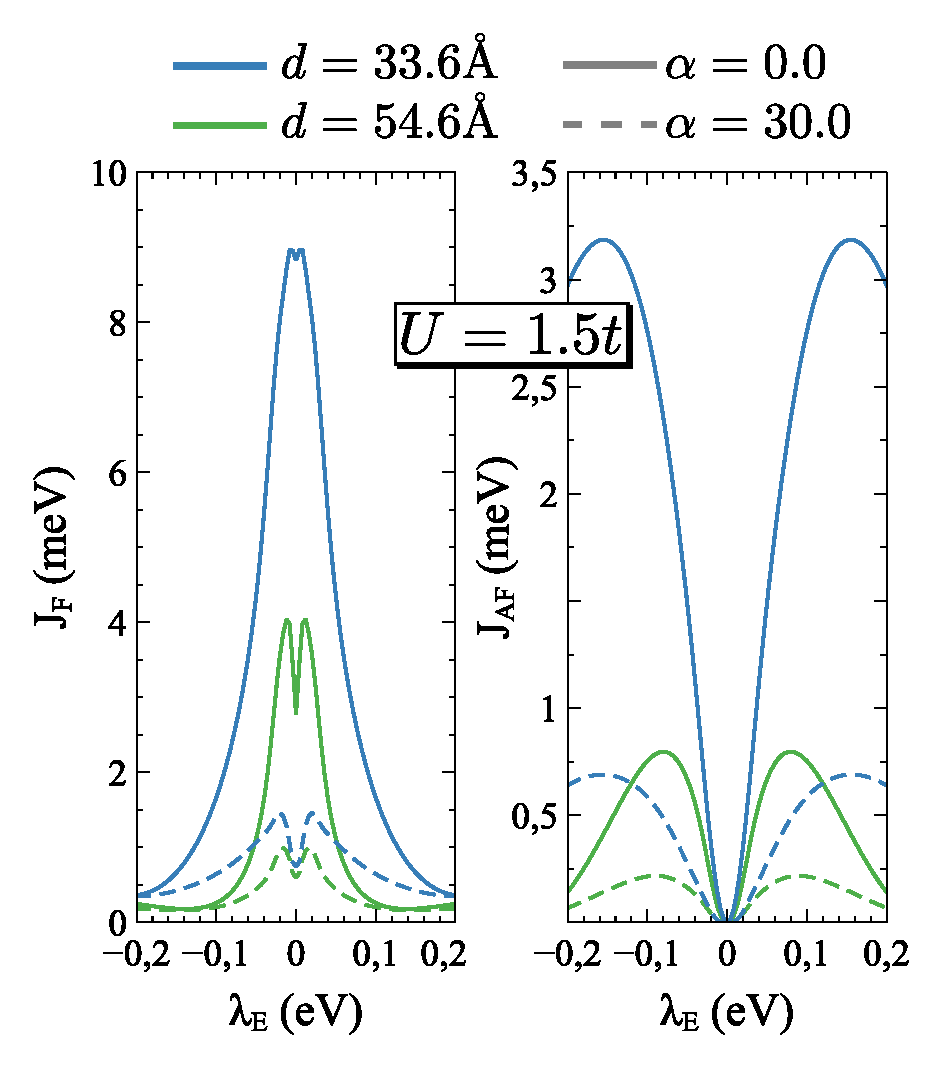
\includegraphics[width=0.7\textwidth]{chapter06/figures/exchange.pdf}
\vspace{-5pt}
\caption{$a)$ shows the dependence of the effective Ferro coupling with the electric field. $b)$ shows the dependence of the effective Anti-Ferro coupling with the electric field.}
\label{exchange}
\end{figure}
\FloatBarrier
%~~~~~~~~~~~~~~~~~~~~~~~~~~~~~~~~~~~~~~~~~~~~~~~~~~~~~~~~~~~%

The shadowed region in Fig.~\ref{exchange} is the same as in Fig.~\ref{IPR_lc} but its interpretation it is a little bit more subtle. It still represents the range of electric fields at which the in-gap states are expected to be spread in a region big enough to be affected by the border effects, but now, this region is not restrictive enough since the there will be a competition between the distance between the vacancies and its distance to the borders (see Fig.~\ref{geo_sketch} $b)$).

In fact for the island used for the calculations in Fig.~\ref{exchange} distances between vacancies bigger than $d\sim 100\text{\AA}$ are to be considered with great caution. For big enough electric fields, of course, there is no problem with the border effects (the states are confined enough).


\subsection{Kondo coupling}
We try now to make apparent a Kondo contribution from the Hubbard term
\begin{equation}
  H_{J_{K}} = J_c \sum_c \vec{S}_z \vec{S}_c + J_v \sum_v \vec{S}_z \vec{S}_v
\end{equation}
These terms will contribute to the decoherence times.

We consider first a single vacancy, and start from eq~\eqref{creation}, only now, since there is only one operator for the in-gap state.
\begin{equation}
  \crea{c}{i\sigma} = \sum_v\psi^*_v(i)\crea{a}{v_\sigma}+
                    \sum_c\psi^*_c(i)\crea{a}{c_\sigma}+
                    Z^*(i)\crea{a}{Z\sigma}
\end{equation}

Now we are interested in the mixing of the in-gap state and the conduction and valence states.
%\sum_v\psi_v(i)\crea{a}{v_\sigma}+\sum_c\psi_c(i)\crea{a}{c_\sigma}+Z^*(i)\crea{a}{Z\sigma}
%\sum_v\psi_v(i)\des{a}{v_\sigma}+\sum_c\psi_c(i)\des{a}{c_\sigma}+Z^*(i)\des{a}{Z\sigma}
\begin{equation}
  \begin{split}
    n_\sigma &= \crea{c}{\sigma}\des{c}{\sigma} =
  \left[\sum_v\psi_v^*\crea{a}{v_\sigma}+\sum_c\psi_c^*\crea{a}{c_\sigma}+Z^*_\sigma\crea{a}{Z\sigma}\right]
  \left[\sum_v\psi_v\des{a}{v_\sigma}+\sum_c\psi_c\des{a}{c_\sigma}+Z_\sigma\des{a}{Z\sigma}\right]=\\
  &=\sum_{vv'}\psi_v^*\psi_{v'}\crea{a}{v_\sigma}\des{a}{v'_\sigma}+
  \sum_{vc}\psi_v^*\psi_c\crea{a}{v_\sigma}\des{a}{c_\sigma}+
  \sum_v\psi_v^*Z_\sigma\crea{a}{v_\sigma}\des{a}{Z\sigma}+\\
  &+\sum_{cv}\psi_c^*\psi_v\crea{a}{c_\sigma}\des{a}{v_\sigma}+
  \sum_{cc'}\psi_c^*\psi_{c'}\crea{a}{c_\sigma}\des{a}{c'_\sigma}+
  \sum_c\psi_c^*Z_\sigma\crea{a}{c_\sigma}\des{a}{Z\sigma}+\\
  &+\sum_v Z^*_\sigma\psi_v\crea{a}{Z\sigma}\des{a}{v_\sigma}+
  \sum_cZ^*_\sigma\psi_c\crea{a}{Z\sigma}\des{a}{c_\sigma}+
  Z^*_\sigma Z_\sigma\crea{a}{Z\sigma}\des{a}{Z\sigma}
  \end{split}
\end{equation}

The full Hubbard term, then reads:
\begin{equation}
  \begin{split}
    n_\uaw n_\daw =&
    \left[\sum_{vv'}\psi_v^*\psi_{v'}\crea{a}{v_\uaw}\des{a}{v'_\uaw}+
    \sum_{vc}\psi_v^*\psi_c\crea{a}{v_\uaw}\des{a}{c_\uaw}+
    \sum_v\psi_v^*Z_\uaw\crea{a}{v_\uaw}\des{a}{Z\uaw}+\right.\\
    &+\sum_{cv}\psi_c^*\psi_v\crea{a}{c_\uaw}\des{a}{v_\uaw}+
    \sum_{cc'}\psi_c^*\psi_{c'}\crea{a}{c_\uaw}\des{a}{c'_\uaw}+
    \sum_c\psi_c^*Z_\uaw\crea{a}{c_\uaw}\des{a}{Z\uaw}+\\
    &\left.+\sum_v Z^*_\uaw\psi_v\crea{a}{Z\uaw}\des{a}{v_\uaw}+
    \sum_cZ^*_\uaw\psi_c\crea{a}{Z\uaw}\des{a}{c_\uaw}+
    Z^*_\uaw Z_\uaw\crea{a}{Z\uaw}\des{a}{Z\uaw}\right]\cdot\\
    &\left[\sum_{vv'}\psi_v^*\psi_{v'}\crea{a}{v_\daw}\des{a}{v'_\daw}+
    \sum_{vc}\psi_v^*\psi_c\crea{a}{v_\daw}\des{a}{c_\daw}+
    \sum_v\psi_v^*Z_\daw\crea{a}{v_\daw}\des{a}{Z\daw}+\right.\\
    &+\sum_{cv}\psi_c^*\psi_v\crea{a}{c_\daw}\des{a}{v_\daw}+
    \sum_{cc'}\psi_c^*\psi_{c'}\crea{a}{c_\daw}\des{a}{c'_\daw}+
    \sum_c\psi_c^*Z_\daw\crea{a}{c_\daw}\des{a}{Z\daw}+\\
    &\left.+\sum_v Z^*_\daw\psi_v\crea{a}{Z\daw}\des{a}{v_\daw}+
    \sum_cZ^*_\daw\psi_c\crea{a}{Z\daw}\des{a}{c_\daw}+
    Z^*_\daw Z_\daw\crea{a}{Z\daw}\des{a}{Z\daw}\right]
  \end{split}
\end{equation}
After expanding all these terms
